\begin{chapterpage}{Multiple and logistic regression}
  \chaptertitle{Multiple and logistic \titlebreak{} regression}
  \label{multipleRegressionAndANOVA}
  \label{multipleAndLogisticRegression}
  \label{ch_regr_mult_and_log}
  \chaptersection{introductionToMultipleRegression}
  \chaptersection{model_selection_section}
  \chaptersection{multipleRegressionModelAssumptions}
  \chaptersection{mario_kart_case_study}
  \chaptersection{logisticRegression}
\end{chapterpage}
\renewcommand{\chapterfolder}{ch_regr_mult_and_log}

\chapterintro{The principles of simple linear regression
  lay the foundation for more sophisticated regression
  models used in a wide range of challenging settings.
  In Chapter~\ref{multipleAndLogisticRegression},
  we explore multiple regression, which introduces the
  possibility of more than one predictor in a linear model,
  and logistic regression,
  a technique for predicting categorical
  outcomes with two levels.}




\section{Introduction to multiple regression}
\label{introductionToMultipleRegression}

\index{multiple regression|seealso{regression}}
\index{regression!multiple|(}
\index{regression|(}

Multiple regression extends simple two-variable regression to the case that still has one response but many predictors (denoted $x_1$, $x_2$, $x_3$, ...). The method is motivated by scenarios where many variables may be simultaneously connected to an output.

\index{data!loans|(}

\newcommand{\loNcomma}{10,000}
\newcommand{\loN}{10000}

We will consider data about loans from the peer-to-peer lender,
Lending Club, which is a data set we first encountered in
Chapters~\ref{ch_intro_to_data}
and~\ref{ch_summarizing_data}.
The loan data includes terms of the loan as well as
information about the borrower.
The outcome variable we would like to better understand
is the interest rate assigned to the loan.
For instance, all other characteristics held constant,
does it matter how much debt someone already has?
Does it matter if their income has been verified?
Multiple regression will help us answer these and other questions.

The data set \data{loans} includes results from \loNcomma{} loans,
and we'll be looking at a subset of the available variables,
some of which will be new from those we saw in earlier chapters.
The first six observations in the data set are shown in
Figure~\ref{loansDataMatrix},
and descriptions for each variable are shown in
Figure~\ref{loansVariables}.
Notice that the past bankruptcy variable (\var{bankruptcy})
is an indicator variable\index{indicator variable},
where it takes the value 1 if the borrower had a past
bankruptcy in their record and 0 if not.
Using an indicator variable in place of a category name
allows for these variables to be directly used in regression.
Two of the other variables are
categorical\index{categorical variable}
(\var{income\us{}ver} and \var{issued}), each of which
can take one of a few different non-numerical values;
we'll discuss how these are handled in the model in
Section~\ref{ind_and_cat_vars_as_predictors}.

\begin{figure}[h]
\centering\footnotesize
\begin{tabular}{r ccc ccc cc}
  \hline
   & interest\us{}rate & income\us{}ver
       & debt\us{}to\us{}income & credit\us{}util
       & bankruptcy & term
       & issued & credit\us{}checks \\ 
  \hline
  1 & 14.07 & verified & 18.01 & 0.55 & 0 & 60 & Mar2018 & 6 \\ 
  2 & 12.61 & not & 5.04 & 0.15 & 1 & 36 & Feb2018 & 1 \\ 
  3 & 17.09 & source\_only & 21.15 & 0.66 & 0 & 36 & Feb2018 & 4 \\ 
  4 & 6.72 & not & 10.16 & 0.20 & 0 & 36 & Jan2018 & 0 \\ 
  5 & 14.07 & verified & 57.96 & 0.75 & 0 & 36 & Mar2018 & 7 \\ 
  6 & 6.72 & not & 6.46 & 0.09 & 0 & 36 & Jan2018 & 6 \\
  $\vdots$ & $\vdots$ & $\vdots$ &
      $\vdots$ & $\vdots$ & $\vdots$ &
      $\vdots$ & $\vdots$ & $\vdots$ \\
   \hline
\end{tabular}
\caption{First six rows from the \data{loans} data set.}
\label{loansDataMatrix}
\end{figure}
%library(openintro)  # Run some example code from loans_full_schema
%library(xtable); xtable(rbind.data.frame(head(d[, c("interest_rate", co)], 6))) #, tail(d[, c("interest_rate", co)], 2)))

\begin{figure}[h]
\centering\small
\begin{tabular}{lp{11.5cm}}
\hline
{\bf variable} & {\bf description} \\
\hline
\var{interest\us{}rate} &
    Interest rate for the loan. \\
\var{income\us{}ver} &
    Categorical variable describing whether the borrower's
    income source and amount have been verified,
    with levels \resp{verified}, \resp{source\us{}only},
    and \resp{not}. \\
\var{debt\us{}to\us{}income} &
    Debt-to-income ratio, which is the percentage of total debt
    of the borrower divided by their total income. \\
\var{credit\us{}util} &
    Of all the credit available to the borrower,
    what fraction are they utilizing.
    For example, the credit utilization on a credit card would
    be the card's balance divided by the card's credit limit. \\
\var{bankruptcy} &
    An indicator variable for whether the borrower has a past
    bankruptcy in her record. This variable takes a value of
    \resp{1} if the answer is ``yes''
    and \resp{0} if the answer is ``no''. \\
\var{term} &
    The length of the loan, in months. \\
\var{issued} &
    The month and year the loan was issued,
    which for these loans is always during the first
    quarter of 2018. \\
\var{credit\us{}checks} &
    Number of credit checks in the last 12 months.
    For example, when filing an application for a credit card,
    it is common for the company receiving the application
    to run a credit check. \\
\hline
\end{tabular}
\caption{Variables and their descriptions for the
    \data{loans} data set.}
\label{loansVariables}
\end{figure}


\newpage

\subsection{Indicator and categorical variables as predictors}
\label{ind_and_cat_vars_as_predictors}

\newcommand{\pastbankrACoef}{0.74}
\newcommand{\pastbankrACoefSE}{0.15}

Let's start by fitting a linear regression model for
interest rate with a single predictor indicating whether
or not a person has a bankruptcy in their record:
\begin{align*}
\widehat{rate} &= 12.33 + \pastbankrACoef{} \times bankruptcy
\end{align*}
Results of this model are shown in
Figure~\ref{intRateVsPastBankrModel}.
%and a scatterplot for price
%versus game condition is shown in
%Figure~\ref{intRateVsPastBankrScatter}.

\begin{figure}[h]
\centering
\begin{tabular}{l rrr r}
  \hline
  \vspace{-3.7mm} & & & & \\
  & Estimate & Std. Error & t value & Pr($>$$|$t$|$) \\ 
  \hline
  (Intercept) & 12.3380 & 0.0533 & 231.49 & $<$0.0001 \\ 
  bankruptcy & 0.7368 & 0.1529 & 4.82 & $<$0.0001 \\ 
  \hline
  &&&\multicolumn{2}{r}{$df=9998$}
\end{tabular}
\caption{Summary of a linear model for predicting
    interest rate based on whether the borrower has
    a bankruptcy in their record.}
\label{intRateVsPastBankrModel}
\end{figure}

%\begin{figure}[h]
%  \centering
%  \Figures{0.45}{loansSingles}{intRateVsPastBankrScatter}
%  \caption{Scatterplot of interest rate against
%      the past bankruptcy indicator variable.
%      The least squares line is also shown,
%      representing a relatively small difference
%      between the two bankruptcy groups.}
%  \label{intRateVsPastBankrScatter}
%\end{figure}

%\begin{exercisewrap}
%\begin{nexercise}
%Examine Figure~\ref{intRateVsPastBankrScatter}.
%Are the conditions for a linear model reasonable?\footnotemark
%\end{nexercise}
%\end{exercisewrap}
%\footnotetext{Yes. Constant variability, nearly normal residuals, and linearity all appear reasonable.}

\begin{examplewrap}
\begin{nexample}{Interpret the coefficient for the
     past bankruptcy variable in the model.
     Is this coefficient significantly different from 0?}
  The \var{bankruptcy} variable takes one of two values:
  1 when the borrower has a bankruptcy
  in their history and 0 otherwise.
  A slope of \pastbankrACoef{} means that the model predicts a
  \pastbankrACoef{}\% higher
  interest rate for those borrowers with a bankruptcy in
  their record.
  (See Section~\ref{categoricalPredictorsWithTwoLevels}
  for a review of the interpretation for two-level
  categorical predictor variables.)
  Examining the regression output in
  Figure~\ref{intRateVsPastBankrModel},
  we can see that the p-value for \var{bankruptcy}
  is very close to zero, indicating there is strong evidence
  the coefficient is different from zero when using this
  simple one-predictor model.
\end{nexample}
\end{examplewrap}

Suppose we had fit a model using a 3-level categorical variable,
such as \var{income\us{}ver}.
The output from software is shown in
Figure~\ref{intRateVsVerIncomeModel}.
This regression output provides multiple
rows for the \var{income\us{}ver} variable.
Each row represents the relative difference for
each level of \var{income\us{}ver}.
However, we are missing one of the levels:
\resp{not} (for \emph{not verified}).
The missing level is called the \term{reference level},
and it represents the default level that
other levels are measured against.
%This will make more sense after we write out the equation.

\begin{figure}[h]
\centering
\begin{tabular}{l rrr r}
  \hline
  \vspace{-3.7mm} & & & & \\
  & Estimate & Std. Error & t value & Pr($>$$|$t$|$) \\ 
  \hline
  (Intercept) &
      11.0995 & 0.0809 & 137.18 & $<$0.0001 \\
  income\us{}ver\lmlevel{source\us{}only} &
      1.4160 & 0.1107 & 12.79 & $<$0.0001 \\ 
  income\us{}ver\lmlevel{verified} &
      3.2543 & 0.1297 & 25.09 & $<$0.0001 \\ 
  \hline
  &&&\multicolumn{2}{r}{$df=9998$}
\end{tabular}
\caption{Summary of a linear model for predicting
    interest rate based on whether the borrower's
    income source and amount has been verified.
    This predictor has three levels, which results
    in 2 rows in the regression output.}
\label{intRateVsVerIncomeModel}
\end{figure}

\begin{examplewrap}
\begin{nexample}{How would we write an equation for
    this regression model?}
  \label{verIncomeEquationExample}%
  The equation for the regression model may be written as
  a model with two predictors:
  \begin{align*}
  \widehat{rate} = 11.10 +
      1.42 \times
          \indfunc{income\us{}ver}{source\us{}only} +
      3.25 \times
          \indfunc{income\us{}ver}{verified}
  \end{align*}
  We use the notation $\indfunc{variable}{level}$
  to represent indicator variables\index{indicator variable}
  for when the categorical variable takes a particular value.
  For example, $\indfunc{income\us{}ver}{source\us{}only}$
  would take a value of 1 if \var{income\us{}ver} was
  \resp{source\us{}only} for a loan,
  and it would take a value of 0 otherwise.
  Likewise, $\indfunc{income\us{}ver}{verified}$ would take
  a value of 1 if \var{income\us{}ver} took a value
  of \resp{verified} and 0 if it took any other value.
  % In Example~\ref{}, we'll run through a few examples
  % of how we can use the equation for the model.
\end{nexample}
\end{examplewrap}

The notation used in Example~\ref{verIncomeEquationExample}
may feel a bit confusing.
Let's figure out how to use the equation for each level
of the \var{income\us{}ver} variable.

\begin{examplewrap}
\begin{nexample}{Using the model from
    Example~\ref{verIncomeEquationExample},
    compute the average interest rate for borrowers
    whose income source and amount are both unverified.}
  When \var{income\us{}ver} takes a value of \resp{not},
  then both indicator functions in the equation from
  Example~\ref{verIncomeEquationExample}
  are set to zero:
  \begin{align*}
  \widehat{rate} &= 11.10 +
      1.42 \times 0 +
      3.25 \times 0 \\
    &= 11.10
  \end{align*}
  The average interest rate for these borrowers is 11.1\%.
  Because the \resp{not} level does not have its own
  coefficient and it is the reference value,
  the indicators for the other levels for this variable
  all drop out.
\end{nexample}
\end{examplewrap}

\begin{examplewrap}
\begin{nexample}{Using the model from
    Example~\ref{verIncomeEquationExample},
    compute the average interest rate for borrowers
    whose income source is verified but the amount is not.}
  When \var{income\us{}ver} takes a value of
  \resp{source\us{}only},
  then the corresponding variable takes a value of 1
  while the other ($\indfunc{income\us{}ver}{verified}$) is 0:
  \begin{align*}
  \widehat{rate} &= 11.10 +
      1.42 \times 1 +
      3.25 \times 0 \\
    &= 12.52
  \end{align*}
  The average interest rate for these borrowers is 12.52\%.
\end{nexample}
\end{examplewrap}

\begin{exercisewrap}
\begin{nexercise}
Compute the average interest rate for borrowers
whose income source and amount are both verified.\footnotemark
\end{nexercise}
\end{exercisewrap}
\footnotetext{When \var{income\us{}ver} takes a value of
  \resp{verified},
  then the corresponding variable takes a value of 1
  while the other ($\indfunc{income\us{}ver}{source\us{}only}$)
  is~0:
  \begin{align*}
  \widehat{rate} &= 11.10 +
      1.42 \times 0 +
      3.25 \times 1 \\
    &= 14.35
  \end{align*}
  The average interest rate for these borrowers is 14.35\%.}

\begin{onebox}{Predictors with several categories}
When fitting a regression model with a categorical variable
that has $k$ levels where $k > 2$, software will provide
a coefficient for $k - 1$ of those levels.
For the last level that does not receive a coefficient,
this is the \term{reference level}, and the coefficients
listed for the other levels are all considered relative
to this reference level.
\end{onebox}

\D{\newpage}

\begin{exercisewrap}
\begin{nexercise}
Interpret the coefficients in the \var{income\us{}ver}
model.\footnotemark
\end{nexercise}
\end{exercisewrap}
\footnotetext{Each of the coefficients gives the
  incremental interest rate for the corresponding level
  relative to the \resp{not} level, which is the reference
  level.
  For example, for a borrower whose income source and
  amount have been verified, the model predicts that
  they will have a 3.25\% higher interest rate than
  a borrower who has not had their income source or
  amount verified.}

The higher interest rate for borrowers who have verified
their income source or amount is surprising.
Intuitively, we'd think that a loan would look \emph{less}
risky if the borrower's income has been verified.
However, note that the situation may be more complex,
and there may be confounding variables
that we didn't account for.
For example, perhaps lender require borrowers with
poor credit to verify their income.
That is, verifying income in our data set might be
a signal of some concerns about the borrower
rather than a reassurance that the borrower will pay
back the loan.
For this reason, the borrower could be deemed higher
risk, resulting in a higher interest rate.
(What other confounding variables might explain this
counter-intuitive relationship suggested by the model?)

\begin{exercisewrap}
\begin{nexercise}
How much larger of an interest rate would we expect for
a borrower who has verified their income source and amount
vs a borrower whose income source has only been
verified?\footnotemark
\end{nexercise}
\end{exercisewrap}
\footnotetext{Relative to the \resp{not} category,
  the \resp{verified} category has an interest rate of
  3.25\% higher, while the \resp{source\us{}only}
  category is only 1.42\% higher.
  Thus, \resp{verified} borrowers will tend to get
  an interest rate about $3.25\% - 1.42\% = 1.83\%$
  higher than \resp{source\us{}only} borrowers.}


\subsection{Including and assessing many variables in a model}
\label{includingAndAssessingManyVariablesInAModel}

The world is complex, and it can be helpful to
consider many factors at once in statistical modeling.
For example, we might like to use the full context of
borrower to predict the interest rate they receive
rather than using a single variable.
This is the strategy used in
\termsub{multiple regression}{regression!multiple}.
While we remain cautious about making any causal
interpretations using multiple regression
on observational data,
such models are a common first step in gaining insights
or providing some evidence of a causal connection.

We want to construct a model that accounts for not only
for any past bankruptcy or whether the borrower had
their income source or amount verified,
but simultaneously accounts for all the variables
in the data set:
\var{income\us{}ver},
\var{debt\us{}to\us{}income},
\var{credit\us{}util},
\var{bankruptcy},
\var{term},
\var{issued},
and \var{credit\us{}checks}.
\begin{align*}
\widehat{\var{rate}}
	&= \beta_0 +
	    \beta_1\times \indfunc{income\us{}ver}{source\us{}only} +
	    \beta_2\times \indfunc{income\us{}ver}{verified} +
		\beta_3\times \var{debt\us{}to\us{}income} \\
	&\qquad\  +
	    \beta_4 \times \var{credit\us{}util} +
	    \beta_5 \times \var{bankruptcy} +
		\beta_6 \times \var{term} \\
	&\qquad\  +
	    \beta_7 \times \indfunc{issued}{Jan2018} +
	    \beta_8 \times \indfunc{issued}{Mar2018} +
		\beta_9 \times \var{credit\us{}checks}
\end{align*}
This equation represents a holistic approach for modeling
all of the variables simultaneously.
Notice that there are two coefficients for \var{income\us{}ver}
and also two coefficients for \var{issued}, since both are
3-level categorical variables.

%\Comment{Work on this paragraph.}
%A multiple regression model may be missing important components or it might not precisely represent the relationship between the outcome and the available explanatory variables. While no model is perfect, we wish to explore the possibility that this one may fit the data reasonably well.


We estimate the parameters
$\beta_0$, $\beta_1$, $\beta_2$, ..., $\beta_9$
in the same way as we did in the case of a single predictor.
We select $b_0$, $b_1$, $b_2$, ..., $b_9$ that minimize the
sum of the squared residuals:
\begin{align}\label{sumOfSqResInMultRegr}
SSE = e_1^2 + e_2^2 + \dots + e_{\loN}^2
	= \sum_{i=1}^{\loN} e_i^2
	 = \sum_{i=1}^{\loN} \left(y_i - \hat{y}_i\right)^2
\end{align}
where $y_i$ and $\hat{y}_i$ represent the observed
interest rates and their estimated values according to
the model, respectively.
\loNcomma{} residuals are calculated, one for each observation.
We typically use a computer to minimize the sum of squares
and compute point estimates, as shown in the sample output
in Figure~\ref{loansFullModelOutput}.
Using this output, we identify the point estimates $b_i$ of
each $\beta_i$, just as we did in the one-predictor case.

\newcommand{\pastbankrFullCoef}{0.39}
\newcommand{\pastbankrFullCoefSE}{0.13}

\begin{figure}[ht]
\centering
\begin{tabular}{rrrrr}
  \hline
  \vspace{-3.7mm} & & & & \\
  & Estimate & Std. Error & t value & Pr($>$$|$t$|$) \\ 
  \hline
  \vspace{-3.8mm} & & & & \\
  (Intercept) & 1.9251 & 0.2102 & 9.16 & $<$0.0001 \\ 
  income\us{}ver\lmlevel{source\us{}only} &
      0.9750 & 0.0991 & 9.83 & $<$0.0001 \\ 
  income\us{}ver\lmlevel{verified} &
      2.5374 & 0.1172 & 21.65 & $<$0.0001 \\ 
  debt\us{}to\us{}income & 0.0211 & 0.0029 & 7.18 & $<$0.0001 \\ 
  credit\us{}util & 4.8959 & 0.1619 & 30.24 & $<$0.0001 \\ 
  bankruptcy & 0.3864 & 0.1324 & 2.92 & 0.0035 \\ 
  term & 0.1537 & 0.0039 & 38.96 & $<$0.0001 \\ 
  issued\lmlevel{Jan2018} & 0.0276 & 0.1081 & 0.26 & 0.7981 \\ 
  issued\lmlevel{Mar2018} & -0.0397 & 0.1065 & -0.37 & 0.7093 \\ 
  credit\us{}checks & 0.2282 & 0.0182 & 12.51 & $<$0.0001 \\ 
   \hline
   &&&\multicolumn{2}{r}{$df=9990$}
\end{tabular}
\caption{Output for the regression model, where
    \var{interest\us{}rate} is the outcome and
    the variables listed are the predictors.}
\label{loansFullModelOutput}
\end{figure}

\begin{onebox}{Multiple regression model}
  A multiple regression model is a linear model
  with many predictors.
  In general, we write the model as
  \begin{align*}
  \hat{y} =
      \beta_0 + \beta_1 x_1 + \beta_2 x_2 + \cdots + \beta_k x_k
  \end{align*}
  when there are $k$ predictors.
  We always estimate the $\beta_i$ parameters using
  statistical software.
\end{onebox}

\begin{examplewrap}
\begin{nexample}{Write out the regression model using
    the point estimates from
    Figure~\ref{loansFullModelOutput}.
    How many predictors are there in this model?}
  \label{loansFullModelEqWCoef}%
  The fitted model for the interest rate is given by:
  {\small\begin{align*}
  \widehat{\var{rate}}
	&= 1.925 +
	    0.975 \times \indfunc{income\us{}ver}{source\us{}only} +
	    2.537 \times \indfunc{income\us{}ver}{verified} +
		0.021 \times \var{debt\us{}to\us{}income} \\
	&\qquad\  +
	    4.896 \times \var{credit\us{}util} +
	    0.386 \times \var{bankruptcy} +
		0.154 \times \var{term} \\
	&\qquad\  +
	    0.028 \times \indfunc{issued}{Jan2018}
	    -0.040 \times \indfunc{issued}{Mar2018} +
		0.228 \times \var{credit\us{}checks}
  \end{align*}}%
  If we count up the number of predictor coefficients,
  we get the \emph{effective} number of predictors
  in the model:~$k = 9$.
  Notice that the \var{issued} categorical predictor
  counts as two, once for the two levels shown in the model.
  In general, a categorical predictor with $p$ different
  levels will be represented by $p - 1$ terms in a multiple
  regression model.
\end{nexample}
\end{examplewrap}


\begin{exercisewrap}
\begin{nexercise}
What does $\beta_4$, the coefficient of variable
\var{credit\us{}util}, represent?
What is the point estimate of~$\beta_4$?\footnotemark
\end{nexercise}
\end{exercisewrap}
\footnotetext{$\beta_4$ represents the change in
   interest rate we would expect if someone's credit
   utilization was 0 and went to 1,
   all other factors held even.
   The point estimate is $b_4 = 4.90\%$.}

\D{\newpage}

\begin{examplewrap}
\begin{nexample}{Compute the residual of the first observation
    in Figure~\ref{loansDataMatrix} on
    page~\pageref{loansDataMatrix} using the equation identified
    in Guided Practice~\ref{loansFullModelEqWCoef}.}
  To compute the residual, we first need the predicted value,
  which we compute by plugging values into the equation from
  Example~\ref{loansFullModelEqWCoef}.
  For example, $\indfunc{income\us{}ver}{source\us{}only}$
  takes a value of 0,
  $\indfunc{income\us{}ver}{verified}$ takes a value of 1
  (since the borrower's income source and amount were verified),
  \var{debt\us{}to\us{}income} was 18.01, and so on.
  This leads to a prediction of $\widehat{rate}_1 = 18.09$.
  The observed interest rate was 14.07\%, which leads to
  a residual of $e_1 = 14.07 - 18.09 = -4.02$.
\end{nexample}
\end{examplewrap}
% sum(model.matrix(m)[1, ] * round(m$coef, 3))

\begin{examplewrap}
\begin{nexample}{We estimated a coefficient for
    \var{bankruptcy} in
    Section~\ref{ind_and_cat_vars_as_predictors}
    of $b_4 = \pastbankrACoef{}$ with a standard error
    of $SE_{b_1} = \pastbankrACoefSE{}$ when using simple
    linear regression.
    Why is there be a difference between that estimate
    and the estimated coefficient of \pastbankrFullCoef{}
    in the multiple regression setting?}
  \label{pastBankrCoefDiffExplained}%
  If we examined the data carefully, we would see that
  some predictors are correlated.
  For instance, when we estimated the connection of the
  outcome \var{interest\us{}rate} and predictor
  \var{bankruptcy} using simple linear regression,
  we were unable to control for other variables like
  whether the borrower had her income verified,
  the borrower's debt-to-income ratio, and other variables.
  That original model was constructed in a vacuum and did
  not consider the full context.
  When we all of the variables, underlying and unintentional
  bias that was missed by these other variables is reduced
  or eliminated.
  Of course, bias can still exist from other confounding
  variables.
\end{nexample}
\end{examplewrap}

Example~\ref{pastBankrCoefDiffExplained} describes a common
issue in multiple regression: correlation among predictor
variables.
We say the two predictor variables are \term{collinear}
(pronounced as \emph{co-linear}) when they are correlated,
and this collinearity complicates model estimation.
While it is impossible to prevent collinearity from arising
in observational data, experiments are usually designed to
prevent predictors from being collinear.

\begin{exercisewrap}
\begin{nexercise}
The estimated value of the intercept is 1.925, and one might
be tempted to make some interpretation of this coefficient,
such as, it is the model's predicted price when each of the
variables take value zero: income source is not verified,
the borrower has no debt (debt-to-income and credit
utilization are zero), and so on.
Is this reasonable?
Is there any value gained by making this
interpretation?\footnotemark
\end{nexercise}
\end{exercisewrap}
\footnotetext{Many of the variables do take a value 0
  for at least one data point, and for those variables,
  it is reasonable.
  However, one variable never takes a value of zero:
  \var{term}, which describes the length of the loan,
  in months.
  If \var{term} is set to zero, then the loan
  must be paid back immediately; the borrower
  must give the money back as soon as she receives it,
  which means it is not a real loan.
  Ultimately, the interpretation of the intercept in
  this setting is not insightful.}


\D{\newpage}

\subsection[Adjusted $R^2$ as a better tool
    for multiple regression]
    {Adjusted $\pmb{R^2}$ as a better tool
        for multiple regression}

\index{adjusted r squared@adjusted $R^2$ ($R_{adj}^2$)|(}

We first used $R^2$ in Section~\ref{fittingALineByLSR}
to determine the amount of variability in the response
that was explained by the model:
\begin{align*}
R^2 =
    1 - \frac{\text{variability in residuals}}
        {\text{variability in the outcome}}
	= 1 - \frac{Var(e_i)}{Var(y_i)}
\end{align*}
where $e_i$ represents the residuals of the model and
$y_i$ the outcomes.
This equation remains valid in the multiple regression
framework, but a small enhancement can make it even
more informative when comparing models.

\begin{exercisewrap}
\begin{nexercise}
\label{computeUnadjR2ForFullLoansModel}%
The variance of the residuals for the model given in
Guided Practice~\ref{loansFullModelEqWCoef}
is 18.53, and the variance of the total price in all
the auctions is 25.01.
Calculate $R^2$ for this model.\footnotemark
\end{nexercise}
\end{exercisewrap}
\footnotetext{$R^2 = 1 - \frac{18.53}{25.01} = 0.2591$.}

This strategy for estimating $R^2$ is acceptable when there
is just a single variable.
However, it becomes less helpful when there are many
variables.
The regular $R^2$ is a biased estimate of the amount of
variability explained by the model
when applied to a new sample of data.
To get a better estimate, we use the adjusted $R^2$.

\begin{onebox}{Adjusted $\pmb{R^2}$ as a tool for
    model assessment}
  The \termsub{adjusted $\pmb{R^2}$}
      {adjusted r squared@adjusted $R^2$ ($R_{adj}^2$)}
  is computed as
  \begin{align*}
  R_{adj}^{2}
    = 1 - \frac{s_{\text{residuals}}^2 / (n-k-1)}
        {s_{\text{outcome}}^2 / (n-1)}
    = 1 - \frac{s_{\text{residuals}}^2}{s_{\text{outcome}}^2}
        \times \frac{n-1}{n-k-1}
  \end{align*}
  where $n$ is the number of cases used to fit the model
  and $k$ is the number of predictor variables in the model.
  Remember that a categorical predictor with $p$ levels will
  contribute $p - 1$ to the number of variables in the model.
\end{onebox}

Because $k$ is never negative, the adjusted $R^2$ will be
smaller -- often times just a little smaller -- than the
unadjusted $R^2$.
The reasoning behind the adjusted $R^2$ lies in the
\termsub{degrees of freedom}{degrees of freedom (df)!regression}
associated with each variance,
which is equal to $n - k - 1$ for the multiple regression
context.
If we were to make predictions for \emph{new data}
using our current model, we would find that the unadjusted
$R^2$ would tend to be slightly overly optimistic, while
the adjusted $R^2$ formula helps correct this bias.

\begin{exercisewrap}
\begin{nexercise}
There were $n=10000$ auctions in the \data{loans} data set
and $k=9$ predictor variables in the model.
Use $n$, $k$, and the variances from
Guided Practice~\ref{computeUnadjR2ForFullLoansModel}
to calculate $R_{adj}^2$ for the interest rate
model.\footnotemark
\end{nexercise}
\end{exercisewrap}
\footnotetext{$R_{adj}^2
    = 1 - \frac{18.53}{25.01}\times \frac{10000-1}{1000-9-1}
    = 0.2584$.
  While the difference is very small, it will be important
  when we fine tune the model in the next section.}

\begin{exercisewrap}
\begin{nexercise}
Suppose you added another predictor to the model, but the
variance of the errors $Var(e_i)$ didn't go down.
What would happen to the~$R^2$?
What would happen to the
adjusted~$R^2$?\hspace{0.7mm}\footnotemark
\end{nexercise}
\end{exercisewrap}
\footnotetext{The unadjusted $R^2$ would stay the same
    and the adjusted $R^2$ would go down.}

Adjusted $R^2$ could have been used in
Chapter~\ref{linRegrForTwoVar}.
However, when there is only $k = 1$ predictors,
adjusted $R^2$ is very close to regular $R^2$,
so this nuance isn't typically important when
the model has only one predictor.

\index{adjusted r squared@adjusted $R^2$ ($R_{adj}^2$)|)}


{


%_______________
\newpage\subsection*{Exercises} % Introduction to multiple regression

% 1

\eoce{\qt{Baby weights, Part I\label{baby_weights_smoke}} The Child Health 
and Development Studies investigate a range of topics. One study 
considered all pregnancies between 1960 and 1967 among women in the 
Kaiser Foundation Health Plan in the San Francisco East Bay area. Here, 
we study the relationship between smoking and weight of the baby. The 
variable \texttt{smoke} is coded 1 if the mother is a smoker, and 0 if 
not. The summary table below shows the results of a linear regression 
model for predicting the average birth weight of babies, measured in 
ounces, based on the smoking status of the mother. 
\footfullcite{data:babies}
\begin{center}
\begin{tabular}{rrrrr}
  \hline
            & Estimate  & Std. Error  & t value   & Pr($>$$|$t$|$) \\ 
  \hline
(Intercept) & 123.05    & 0.65        & 189.60    & 0.0000 \\ 
smoke       & -8.94     & 1.03        & -8.65     & 0.0000 \\ 
  \hline
\end{tabular}
\end{center}
The variability within the smokers and non-smokers are about equal and the 
distributions are symmetric. With these conditions satisfied, it is reasonable 
to apply the model. (Note that we don't need to check linearity since the 
predictor has only two levels.)
\begin{parts}
\item Write the equation of the regression model.
\item Interpret the slope in this context, and calculate the predicted birth 
weight of babies born to smoker and non-smoker mothers.
\item Is there a statistically significant relationship between the average birth 
weight and smoking?
\end{parts}
}{}

% 2

\eoce{\qt{Baby weights, Part II\label{baby_weights_parity}} 
Exercise~\ref{baby_weights_smoke} introduces a data set on birth weight of 
babies. Another variable we consider is \texttt{parity}, which is 0 if the child 
is the first born, and 1 otherwise. The summary table below shows the results of 
a linear regression model for predicting the average birth weight of babies, 
measured in ounces, from \texttt{parity}. 
\begin{center}
\begin{tabular}{rrrrr}
  \hline
            & Estimate  & Std. Error    & t value   & Pr($>$$|$t$|$) \\ 
  \hline
(Intercept) & 120.07    & 0.60        & 199.94    & 0.0000 \\ 
parity      	& -1.93     	  & 1.19        & -1.62       & 0.1052 \\ 
  \hline
\end{tabular}
\end{center}
\begin{parts}
\item Write the equation of the regression model.
\item Interpret the slope in this context, and calculate the predicted birth 
weight of first borns and others.
\item Is there a statistically significant relationship between the average 
birth weight and parity?
\end{parts}
}{}

% 3

\eoce{\qt{Baby weights, Part III\label{baby_weights_mlr}} We considered the 
variables \texttt{smoke} and \texttt{parity}, one at a time, in modeling birth 
weights of babies in Exercises~\ref{baby_weights_smoke} and~\ref{baby_weights_parity}. 
A more realistic approach to modeling infant 
weights is to consider all possibly related variables at once. Other variables 
of interest include length of pregnancy in days (\texttt{gestation}), mother's 
age in years (\texttt{age}), mother's height in inches (\texttt{height}), and 
mother's pregnancy weight in pounds (\texttt{weight}). Below are three 
observations from this data set. 
\begin{center}
\begin{tabular}{r c c c c c c c}
  \hline
      & bwt & gestation & parity  & age   & height  & weight  & smoke \\ 
  \hline
1     & 120 & 284       & 0       & 27    &  62     & 100     &   0 \\ 
2     & 113 & 282       & 0       & 33    &  64     & 135     &   0 \\ 
$\vdots$ & $\vdots$ & $\vdots$ & $\vdots$ &  $\vdots$ & $\vdots$ & $\vdots$ &   $\vdots$ \\ 
1236  & 117 & 297       & 0       & 38    &  65     & 129     &   0 \\ 
   \hline
\end{tabular}
\end{center}
The summary table below shows the results of a regression model for predicting 
the average birth weight of babies based on all of the variables included in 
the data set.
\begin{center}
\begin{tabular}{rrrrr}
  \hline
            & Estimate  & Std. Error  & t value   & Pr($>$$|$t$|$) \\ 
  \hline
(Intercept) & -80.41    & 14.35       & -5.60     & 0.0000 \\ 
gestation   & 0.44      & 0.03        & 15.26     & 0.0000 \\ 
parity      & -3.33     & 1.13        & -2.95     & 0.0033 \\ 
age         & -0.01     & 0.09        & -0.10     & 0.9170 \\ 
height      & 1.15      & 0.21        & 5.63      & 0.0000 \\ 
weight      & 0.05      & 0.03        & 1.99      & 0.0471 \\ 
smoke       & -8.40     & 0.95        & -8.81     & 0.0000 \\ 
  \hline
\end{tabular}
\end{center}
\begin{parts}
\item Write the equation of the regression model that includes all of the 
variables.
\item Interpret the slopes of \texttt{gestation} and \texttt{age} in this 
context.
\item The coefficient for \texttt{parity} is different than in the linear 
model shown in Exercise~\ref{baby_weights_parity}. Why might there be a difference?
\item Calculate the residual for the first observation in the data set.
\item The variance of the residuals is 249.28, and the variance of the birth 
weights of all babies in the data set is 332.57. Calculate the $R^2$ and the 
adjusted $R^2$. Note that there are 1,236 observations in the data set.
\end{parts}
}{}

% 4

\eoce{\qt{Absenteeism, Part I\label{absent_from_school_mlr}} Researchers interested in the 
relationship between absenteeism from school and certain demographic 
characteristics of children collected data from 146 randomly sampled students 
in rural New South Wales, Australia, in a particular school year. Below are 
three observations from 
this data set. 
\begin{center}
\begin{tabular}{r c c c c}
  \hline
 	  & eth 	& sex 	& lrn 	& days \\   
  \hline
1 	& 0 		& 1 		& 1 		&   2 \\ 
2 	& 0 		& 1 		& 1 		&  11 \\ 
$\vdots$ & $\vdots$ & $\vdots$ & $\vdots$ & $\vdots$ \\ 
146 & 1 		& 0 		& 0 		&  37 \\ 
  \hline
\end{tabular}
\end{center}
The summary table below shows the results of a linear regression model for 
predicting the average number of days absent based on ethnic background 
(\texttt{eth}: 0 - aboriginal, 1 - not aboriginal), sex (\texttt{sex}: 0 - 
female, 1 - male), and learner status (\texttt{lrn}: 0 - average learner, 1 - 
slow learner). \footfullcite{data:quine}
\begin{center}
\begin{tabular}{rrrrr}
  \hline
            & Estimate  & Std. Error  & t value   & Pr($>$$|$t$|$) \\ 
  \hline
(Intercept) & 18.93     & 2.57        & 7.37      & 0.0000 \\ 
eth         & -9.11     & 2.60        & -3.51     & 0.0000 \\ 
sex         & 3.10      & 2.64        & 1.18      & 0.2411 \\ 
lrn         & 2.15      & 2.65        & 0.81      & 0.4177 \\ 
  \hline
\end{tabular}
\end{center}
\begin{parts}
\item Write the equation of the regression model.
\item Interpret each one of the slopes in this context.
\item Calculate the residual for the first observation in the data set: a 
student who is aboriginal, male, a slow learner, and missed 2 days of school.
\item The variance of the residuals is 240.57, and the variance of the number of 
absent days for all students in the data set is 264.17. Calculate the $R^2$ and 
the adjusted $R^2$. Note that there are 146 observations in the data set.
\end{parts}
}{}

% 5

\eoce{\qt{GPA\label{gpa}} A survey of 55 Duke University students asked about their 
GPA, number of hours they study at night, number of nights they go out, and 
their gender. Summary output of the regression model is shown below. Note that 
male is coded as 1. 
\begin{center}
\begin{tabular}{rrrrr}
  \hline
            & Estimate  & Std. Error  & t value   & Pr($>$$|$t$|$) \\ 
  \hline
(Intercept) & 3.45      & 0.35        & 9.85      & 0.00 \\ 
studyweek   & 0.00      & 0.00        & 0.27      & 0.79 \\ 
sleepnight  & 0.01      & 0.05        & 0.11      & 0.91 \\ 
outnight    & 0.05      & 0.05        & 1.01      & 0.32 \\ 
gender      & -0.08     & 0.12        & -0.68     & 0.50 \\ 
  \hline
\end{tabular}
\end{center}
\begin{parts}
\item Calculate a 95\% confidence interval for the coefficient of gender in the 
model, and interpret it in the context of the data.
\item Would you expect a 95\% confidence interval for the slope of the remaining 
variables to include 0? Explain
\end{parts}
}{}

% 6

\eoce{\qt{Cherry trees\label{cherry_trees}} Timber yield is approximately equal to the 
volume of a tree, however, this value is difficult to measure without first 
cutting the tree down. Instead, other variables, such as height and diameter, 
may be used to predict a tree's volume and yield. Researchers wanting to 
understand the relationship between these variables for black cherry trees 
collected data from 31 such trees in the Allegheny National Forest, 
Pennsylvania. Height is measured in feet, diameter in inches (at 54 inches above 
ground), and volume in cubic feet.\footfullcite{Hand:1994}
\begin{table}[ht]
\begin{center}
\begin{tabular}{rrrrr}
  \hline
            & Estimate  & Std. Error  & t value   & Pr($>$$|$t$|$) \\ 
  \hline
(Intercept) & -57.99    & 8.64        & -6.71     & 0.00 \\ 
height      & 0.34      & 0.13        & 2.61      & 0.01 \\ 
diameter    & 4.71      & 0.26        & 17.82     & 0.00 \\ 
  \hline
\end{tabular}
\end{center}
\end{table}
\begin{parts}
\item Calculate a 95\% confidence interval for the coefficient of height, and 
interpret it in the context of the data.
\item One tree in this sample is 79 feet tall, has a diameter of 11.3 inches, 
and is 24.2 cubic feet in volume. Determine if the model overestimates or 
underestimates the volume of this tree, and by how much.
\end{parts}
}{}
}






%__________________
\section{Model selection}
\label{model_selection_section}
\label{modelSelection}

\index{model selection|(}

The best model is not always the most complicated.
Sometimes including variables that are not evidently
important can actually reduce the accuracy of predictions.
In this section, we discuss model selection strategies,
which will help us eliminate variables from the model that
are found to be less important.
It's common (and hip, at least in the statistical world)
to refer to models that have undergone such variable pruning
as \term{parsimonious}.

In practice, the model that includes all available explanatory
variables is often referred to as the \term{full model}.
The full model may not be the best model, and if it isn't,
we want to identify a smaller model that is preferable.


\subsection{Identifying variables in the model that may
    not be helpful}

Adjusted $R^2$ describes the strength of a model fit,
and it is a useful tool for evaluating which predictors
are adding value to the model, where \emph{adding value}
means they are (likely) improving the accuracy in
predicting future outcomes.

Let's consider two models, which are shown in
Tables~\ref{loansFullModelModelSelectionSection}
and~\ref{loansModelAllButIssued}.
The first table summarizes the full model since it includes
all predictors, while the second does not include the
\var{issued} variable.

\begin{figure}[ht]
\centering
\begin{tabular}{rrrrr}
  \hline
  \vspace{-3.7mm} & & & & \\
  & Estimate & Std. Error & t value & Pr($>$$|$t$|$) \\ 
  \hline
  \vspace{-3.8mm} & & & & \\
  (Intercept) & 1.9251 & 0.2102 & 9.16 & $<$0.0001 \\ 
  income\us{}ver\lmlevel{source\us{}only} &
      0.9750 & 0.0991 & 9.83 & $<$0.0001 \\ 
  income\us{}ver\lmlevel{verified} &
      2.5374 & 0.1172 & 21.65 & $<$0.0001 \\ 
  debt\us{}to\us{}income & 0.0211 & 0.0029 & 7.18 & $<$0.0001 \\ 
  credit\us{}util & 4.8959 & 0.1619 & 30.24 & $<$0.0001 \\ 
  bankruptcy & 0.3864 & 0.1324 & 2.92 & 0.0035 \\ 
  term & 0.1537 & 0.0039 & 38.96 & $<$0.0001 \\ 
  issued\lmlevel{Jan2018} & 0.0276 & 0.1081 & 0.26 & 0.7981 \\ 
  issued\lmlevel{Mar2018} & -0.0397 & 0.1065 & -0.37 & 0.7093 \\ 
  credit\us{}checks & 0.2282 & 0.0182 & 12.51 & $<$0.0001 \\ 
  \hline
  \multicolumn{3}{l}{$R_{adj}^2 = 0.25843$}&
      \multicolumn{2}{r}{$df=9990$}
\end{tabular}
\caption{The fit for the full regression model,
    including the adjusted $R^2$.}
\label{loansFullModelModelSelectionSection}
\end{figure}

\begin{figure}[ht]
\centering
\begin{tabular}{rrrrr}
  \hline
  \vspace{-3.7mm} & & & & \\
  & Estimate & Std. Error & t value & Pr($>$$|$t$|$) \\ 
  \hline
  \vspace{-3.8mm} & & & & \\
  (Intercept) & 1.9213 & 0.1982 & 9.69 & $<$0.0001 \\ 
  income\us{}ver\lmlevel{source\us{}only} &
      0.9740 & 0.0991 & 9.83 & $<$0.0001 \\ 
  income\us{}ver\lmlevel{verified} &
      2.5355 & 0.1172 & 21.64 & $<$0.0001 \\ 
  debt\us{}to\us{}income & 0.0211 & 0.0029 & 7.19 & $<$0.0001 \\ 
  credit\us{}util & 4.8958 & 0.1619 & 30.25 & $<$0.0001 \\ 
  bankruptcy & 0.3869 & 0.1324 & 2.92 & 0.0035 \\ 
  term & 0.1537 & 0.0039 & 38.97 & $<$0.0001 \\ 
  credit\us{}checks & 0.2283 & 0.0182 & 12.51 & $<$0.0001 \\ 
  \hline
  \vspace{-3.6mm} & & & & \\
  \multicolumn{3}{l}{$R_{adj}^2 = 0.25854$}&
      \multicolumn{2}{r}{$df=9992$}
\end{tabular}
\caption{The fit for the regression model after dropping
   the \var{issued} variable.} %, which represented 3 categories
   % and 2 degrees of freedom.}
\label{loansModelAllButIssued}
\end{figure}

\begin{examplewrap}
\begin{nexample}{Which of the two models is better?}
  We compare the adjusted $R^2$ of each model to determine
  which to choose.
  Since the first model has an $R^2_{adj}$ smaller than
  the $R^2_{adj}$ of the second model, we prefer the second
  model to the first.
\end{nexample}
\end{examplewrap}

Will the model without \var{issued} be better than the
model with \var{issued}?
We~cannot know for sure, but based on the adjusted $R^2$,
this is our best assessment.


\subsection{Two model selection strategies}

Two common strategies for adding or removing variables
in a multiple regression model are called
\emph{backward elimination} and \emph{forward selection}.
These techniques are often referred to as \term{stepwise}
model selection strategies, because they add or delete
one variable at a time as they ``step'' through the
candidate predictors.

\termsub{Backward elimination}{backward elimination}
starts with the model that includes all potential
predictor variables.
Variables are eliminated one-at-a-time from the model
until we cannot improve the adjusted $R^2$.
The strategy within each elimination step is to eliminate
the variable that leads to the largest improvement in
adjusted $R^2$.

\begin{examplewrap}
\begin{nexample}{Results corresponding to the \emph{full model}
    for the \data{loans} data are shown in
    Figure~\ref{loansFullModelModelSelectionSection}.
    How should we proceed under the backward elimination
    strategy?}
  \label{loansBackwardElimEx}%
  Our baseline adjusted $R^2$ from the full model is
  $R^2_{adj} = 0.25843$, and we need to determine whether
  dropping a predictor will improve the adjusted $R^2$.
  To check, we fit models that each drop a different
  predictor, and we record the adjusted $R^2$:
  \begin{center}
  \begin{tabular}{lllll}
  Exclude ... &
      \var{income\us{}ver} &
      \var{debt\us{}to\us{}income} &
      \var{credit\us{}util} &
      \var{bankruptcy} \\
  &
      $R^2_{adj} = 0.22380$ &
      $R^2_{adj} = 0.25468$ &
      $R^2_{adj} = 0.19063$ &
      $R^2_{adj} = 0.25787$ \\
  \\
  &
      \var{term} &
      \var{issued} &
      \var{credit\us{}checks} \\
  &
      $R^2_{adj} = 0.14581$ &
      $R^2_{adj} = 0.25854$ &
      $R^2_{adj} = 0.24689$ \\
  \end{tabular}
  \end{center}
  The model without \var{issued} has the highest adjusted $R^2$
  of 0.25854, higher than the adjusted $R^2$ for the full model.
  Because eliminating \var{issued} leads to a model with
  a higher adjusted $R^2$, we drop \var{issued} from the model.

  Since we eliminated a predictor from the model in the first step,
  we see whether we should eliminate any additional predictors.
  Our baseline adjusted $R^2$ is now $R^2_{adj} = 0.25854$.
  We now fit new models, which consider eliminating each of the
  remaining predictors in addition to \var{issued}:
  \begin{center}
  \begin{tabular}{llll}
  Exclude \var{issued} and ... &
      \var{income\us{}ver} &
      \var{debt\us{}to\us{}income} &
      \var{credit\us{}util} \\
  &
      $R^2_{adj} = 0.22395$ &
      $R^2_{adj} = 0.25479$ &
      $R^2_{adj} = 0.19074$ \\
  \\
  &
      \var{bankruptcy} &
      \var{term} &
      \var{credit\us{}checks} \\
  &
      $R^2_{adj} = 0.25798$ &
      $R^2_{adj} = 0.14592$ &
      $R^2_{adj} = 0.24701$ \\
  \end{tabular}
  \end{center}
  None of these models lead to an improvement in adjusted $R^2$,
  so we do not eliminate any of the remaining predictors.
  That is, after backward elimination, we are left with the
  model that keeps all predictors except \var{issued},
  which we can summarize using the coefficients from
  Figure~\ref{loansModelAllButIssued}:
  \begin{align*}
  \widehat{rate} &= \ 1.921
      + 0.974 \times \indfunc{income\us{}ver}{source\us{}only}
      + 2.535 \times \indfunc{income\us{}ver}{verified} \\
    &\qquad
      + 0.021 \times \var{debt\us{}to\us{}income}
      + 4.896 \times \var{credit\us{}util}
      + 0.387 \times \var{bankruptcy} \\
    &\qquad
      + 0.154 \times \var{term}
      + 0.228 \times \var{credit\us{}check}
  \end{align*}
\end{nexample}
\end{examplewrap}

The \term{forward selection} strategy is the reverse of the backward elimination technique. Instead of eliminating variables one-at-a-time, we add variables one-at-a-time until we cannot find any variables that improve the model (as measured by adjusted $R^2$).

\begin{examplewrap}
\begin{nexample}{Construct a model for the \data{loans} data
    set using the forward selection strategy.}
  \label{loansForwardElimEx}%
  We start with the model that includes no variables.
  Then we fit each of the possible models with just one
  variable.
  That is, we fit the model including just \var{income\us{}ver},
  then the model including just \var{debt\us{}to\us{}income},
  then a model with just \var{credit\us{}util}, and so on.
  Then we examine the adjusted $R^2$ for each of these models:
  \begin{center}
  \begin{tabular}{lllll}
  Add ... &
      \var{income\us{}ver} &
      \var{debt\us{}to\us{}income} &
      \var{credit\us{}util} &
      \var{bankruptcy} \\
  &
      $R^2_{adj} = 0.05926$ &
      $R^2_{adj} = 0.01946$ &
      $R^2_{adj} = 0.06452$ &
      $R^2_{adj} = 0.00222$ \\
  \\
  &
      \var{term} &
      \var{issued} &
      \var{credit\us{}checks} \\
  &
      $R^2_{adj} = 0.12855$ &
      $R^2_{adj} = -$<$0.00018$ &
      $R^2_{adj} = 0.01711$ \\
  \end{tabular}
  \end{center}
  % for (i in 1:7) { m <- lm(F(co, i), data = d);
  %   cat(i, " ", co[i], " ", AdjR2(m), "\n") }
  In this first step, we compare the adjusted $R^2$ against
  a baseline model that has no predictors.
  The no-predictors model always has $R_{adj}^2 = 0$.
  The model with one predictor that has the largest
  adjusted $R^2$ is the model with the \var{term} predictor,
  and because this adjusted $R^2$ is larger than the
  adjusted $R^2$ from the model with no predictors
  ($R_{adj}^2 = 0$), we will add this variable to our model.

  We repeat the process again, this time considering
  2-predictor models where one of the predictors is
  \var{term} and with a new baseline of $R^2_{adj} = 0.12855$:
  \begin{center}
  \begin{tabular}{llll}
  Add \var{term} and ... &
      \var{income\us{}ver} &
      \var{debt\us{}to\us{}income} &
      \var{credit\us{}util} \\
  &
      $R^2_{adj} = 0.16851$ &
      $R^2_{adj} = 0.14368$ &
      $R^2_{adj} = 0.20046$ \\
  \\
  &
      \var{bankruptcy} &
      \var{issued} &
      \var{credit\us{}checks} \\
  &
      $R^2_{adj} = 0.13070$ &
      $R^2_{adj} = 0.12840$ &
      $R^2_{adj} = 0.14294$ \\
  \end{tabular}
  \end{center}
  The best second predictor, \var{credit\us{}util},
  has a higher adjusted $R^2$ (0.20046) than the
  baseline (0.12855), so we also add \var{credit\us{}util}
  to the model.

  Since we have again added a variable to the model,
  we continue and see whether it would be beneficial
  to add a third variable:
  \begin{center}
  \begin{tabular}{llll}
  Add \var{term}, \var{credit\us{}util}, and ... &
      \var{income\us{}ver} &
      \var{debt\us{}to\us{}income} \\
  &
      $R^2_{adj} = 0.24183$ &
      $R^2_{adj} = 0.20810$ \\
  \\
  &
      \var{bankruptcy} &
      \var{issued} &
      \var{credit\us{}checks} \\
  &
      $R^2_{adj} = 0.20169$ &
      $R^2_{adj} = 0.20031$ &
      $R^2_{adj} = 0.21629$ \\
  \end{tabular}
  \end{center}
  The model adding \var{income\us{}ver} improved adjusted $R^2$
  (0.24183 to 0.20046), so we add \var{income\us{}ver} to the
  model.

  We continue on in this way,
  next adding \var{debt\us{}to\us{}income},
  then \var{credit\us{}checks},
  and \var{bankruptcy}.
  At this point, we come again to the \var{issued} variable:
  adding this variable leads to $R_{adj}^2 = 0.25843$,
  while keeping all the other variables but excluding \var{issued}
  leads to a higher $R_{adj}^2 = 0.25854$.
  This means we do not add \var{issued}.
  In this example, we have arrived at the same model that we
  identified from backward elimination.
\end{nexample}
\end{examplewrap}

\begin{onebox}{Model selection strategies}
  Backward elimination begins with the model
  having the largest number of predictors
  and eliminates variables one-by-one until we are satisfied
  that all remaining variables are important to the model.
  Forward selection starts with no variables included in
  the model, then it adds in variables according to their
  importance until no other important variables are found.
\end{onebox}

Backward elimination and forward selection sometimes
arrive at different final models.
If trying both techniques and this happens, it's common
to choose the model with the larger $R_{adj}^2$.


\subsection{The p-value approach,
    an alternative to adjusted $\pmb{R^2}$}

\noindent%
The p-value may be used as an alternative to $R_{adj}^2$
for model selection:
\begin{description}
\item[Backward elimination with the p-value approach.]
    In backward elimination, we would identify the predictor
    corresponding to the largest p-value.
    If the p-value is above the significance level,
    usually $\alpha = 0.05$, then we would drop that variable,
    refit the model, and repeat the process.
    If the largest p-value is less than $\alpha = 0.05$,
    then we would not eliminate any predictors and the current
    model would be our best-fitting model.
\item[Forward selection with the p-value approach.]
    In forward selection with p-values, we reverse the process.
    We begin with a model that has no predictors, then we fit
    a model for each possible predictor, identifying the model
    where the corresponding predictor's p-value is smallest.
    If that p-value is smaller than $\alpha = 0.05$, we add
    it to the model and repeat the process, considering whether
    to add more variables one-at-a-time.
    When none of the remaining predictors can be added to the
    model and have a p-value less than 0.05,
    then we stop adding variables and the current model would
    be our best-fitting model.
\end{description}

\begin{exercisewrap}
\begin{nexercise}
Examine Figure~\ref{loansModelAllButIssued} on
page~\pageref{loansModelAllButIssued}, which considers the
model including all variables except the variable for the month
the loan was issued.
If we were using the p-value approach with backward elimination
and we were considering this model, which of these variables
would be up for elimination?
Would we drop that variable, or would we keep it in the
model?\footnotemark
\end{nexercise}
\end{exercisewrap}
\footnotetext{The \var{bankruptcy} predictor is up for
  elimination since it has the largest p-value.
  However, since that p-value is smaller than 0.05,
  we would still keep it in the model.}

While the adjusted $R^2$ and p-value approaches are similar,
they sometimes lead to different models, with the $R_{adj}^2$
approach tending to include more predictors in the final model.

\begin{onebox}{Adjusted $\pmb{R^2}$ vs p-value approach}
  When the sole goal is to improve prediction accuracy,
  use $R_{adj}^2$.
  This is commonly the case in machine learning
  applications.\vspace{3mm}

  When we care about understanding which variables are
  statistically significant predictors of the response,
  or if there is interest in producing a simpler model
  at the potential cost of a little prediction accuracy,
  then the p-value approach is preferred.
\end{onebox}

Regardless of whether you use $R_{adj}^2$ or the p-value approach,
or if you use the backward elimination of forward selection
strategy, our job is not done after variable selection.
We must still verify the model conditions are reasonable.

\index{model selection|)}


{\exercisesheader{}

% 7

\eoce{\qt{Baby weights, Part IV\label{baby_weights_model_select_backward}} 
Exercise~\ref{baby_weights_mlr} considers a model that predicts a newborn's 
weight using several predictors (gestation length, parity, age of mother, height 
of mother, weight of mother, smoking status of mother). The table below shows 
the adjusted R-squared for the full model as well as adjusted R-squared values 
for all models we evaluate in the first step of the backwards elimination 
process. 
\begin{center}
\begin{tabular}{rlr}
  \hline
  & Model               & Adjusted $R^2$ \\ 
  \hline
1 & Full model          & 0.2541 \\ 
2 & No gestation        & 0.1031 \\ 
3 & No parity           & 0.2492 \\ 
4 & No age              & 0.2547 \\ 
5 & No height           & 0.2311 \\ 
6 & No weight           & 0.2536 \\ 
7 & No smoking status   & 0.2072 \\ 
  \hline
\end{tabular}
\end{center}
Which, if any, variable should be removed from the model first?
}{}

% 8

\eoce{\qt{Absenteeism, Part II\label{absent_from_school_model_select_backward}} 
Exercise~\ref{absent_from_school_mlr} considers a model that predicts the number 
of days absent using three predictors: ethnic background (\var{eth}), 
gender (\var{sex}), and learner status (\var{lrn}). The table below shows the 
adjusted R-squared for the model as well as adjusted R-squared values for all 
models we evaluate in the first step of the backwards elimination process. 
\begin{center}
\begin{tabular}{rlr}
  \hline
  & Model               & Adjusted $R^2$ \\ 
  \hline
1 & Full model          & 0.0701 \\ 
2 & No ethnicity        & -0.0033 \\ 
3 & No sex              & 0.0676 \\ 
4 & No learner status   & 0.0723 \\ 
  \hline
\end{tabular}
\end{center}
Which, if any, variable should be removed from the model first?
}{}

% 9

\eoce{\qt{Baby weights, Part V\label{baby_weights_model_select_forward}} 
Exercise~\ref{baby_weights_mlr} provides regression output for the full 
model (including all explanatory variables available in the data set) for 
predicting birth weight of babies. In this exercise we consider a forward-
selection algorithm and add variables to the model one-at-a-time. The table 
below shows the p-value and adjusted $R^2$ of each model where we include only 
the corresponding predictor. Based on this table, which variable should be added 
to the model first?\vspace{0.5mm}
\begin{center}
\begin{tabular}{l c c c c c c}
\hline
variable    & gestation	            & parity  & age	    
                & height          
                    & weight              
                        & smoke \\
\hline
p-value	    & $2.2 \times 10^{-16}$	& 0.1052	& 0.2375	
                & $2.97 \times 10^{-12}$
                    & $8.2 \times 10^{-8}$
                        & $2.2 \times 10^{-16}$ \\
$R_{adj}^2$	& 0.1657				        & 0.0013	& 0.0003	
                & 0.0386				
                    & 0.0229				
                        & 0.0569 \\
\hline
\end{tabular}
\end{center}
}{}

% 10

\eoce{\qt{Absenteeism, Part III\label{absent_from_school_model_select_forward}} 
Exercise~\ref{absent_from_school_mlr} provides regression output for the full 
model, including all explanatory variables available in the data set, for 
predicting the number of days absent from school. In this exercise we consider a 
forward-selection algorithm and add variables to the model one-at-a-time. The 
table below shows the p-value and adjusted $R^2$ of each model where we include 
only the corresponding predictor. Based on this table, which variable should be 
added to the model first?\vspace{0.5mm}
\begin{center}
\begin{tabular}{l c c c}
  \hline
variable    & ethnicity  & sex	   & learner status	 \\
  \hline
p-value		& 0.0007     & 0.3142  & 0.5870	 \\
$R_{adj}^2$	& 0.0714     & 0.0001  & 0 \\
  \hline
\end{tabular}
\end{center}
}{}

% 11

\eoce{\qt{Movie lovers, Part I\label{movie_lovers_pval_select}} Suppose a social 
scientist is interested in studying what makes audiences love or hate a movie. 
She collects a random sample of movies (genre, length, cast, director, budget, 
etc.) as well as a measure of the success of the movie (score on a film review 
aggregator website). If as part of her research she is interested in finding out
which variables are significant predictors of movie success, what type of model 
selection method should she use?
}{}

% 12

\eoce{\qt{Movie lovers, Part II\label{movie_lovers_adjrsq_select}} Suppose an online 
media streaming company is interested in building a movie recommendation system. 
The website maintains data on the movies in their database (genre, length, cast, 
director, budget, etc.) and additionally collects data from their subscribers (
demographic information, previously watched movies, how they rated previously 
watched movies, etc.). The recommendation system will be deemed successful if 
subscribers actually watch, and rate highly, the movies recommended to them. 
Should the company use the adjusted $R^2$ or the p-value approach in selecting
variables for their recommendation system?
}{}
}







%%%%%
\section{Checking model conditions using graphs}
\label{multipleRegressionModelAssumptions}

\index{regression!model assumptions|(}
\index{regression!model conditions|(}
\index{regression!technical conditions|(}
\index{regression!conditions|(}

\noindent%
Multiple regression methods using the model
\begin{align*}
\hat{y} &= \beta_0 + \beta_1x_1 + \beta_2x_2 + \cdots + \beta_kx_k
\end{align*}
generally depend on the following four conditions:
\begin{enumerate}
\setlength{\itemsep}{0mm}
\item the residuals of the model are nearly normal
    (less important for larger data sets),
\item the variability of the residuals is nearly constant,
\item the residuals are independent, and
\item each variable is linearly related to the outcome.
\end{enumerate}


\subsection{Diagnostic plots}
\label{diagnostic_plots_subsection}

\termsub{Diagnostic plots}{diagnostic plots} can be used
to check each of these conditions.
We will consider the
model from the Lending Club loans data, and check whether
there are any notable concerns:
\begin{align*}
\widehat{rate} &= \ 1.921
    + 0.974 \times \indfunc{income\us{}ver}{source\us{}only}
    + 2.535 \times \indfunc{income\us{}ver}{verified} \\
  &\qquad
    + 0.021 \times \var{debt\us{}to\us{}income}
    + 4.896 \times \var{credit\us{}util}
    + 0.387 \times \var{bankruptcy} \\
  &\qquad
    + 0.154 \times \var{term}
    + 0.228 \times \var{credit\us{}check}
\end{align*}

\begin{description}
\item[Check for outliers.]
    In theory, the distribution of the residuals should
    be nearly normal;
    in practice, normality can be relaxed for most applications.
    Instead, we examine a histogram of the residuals
    to check if there are any outliers:
    Figure~\ref{loansDiagNormalHistogram}
    is a histogram of these outliers.
    Since this is a very large data set,
    only particularly extreme observations would be a concern
    in this particular case.
    There are no extreme observations that might cause a~concern.

    If we intended to construct what are called
    \termsub{prediction intervals}{prediction interval}
    for future observations,
    we would be more strict and
    require the residuals to be nearly normal.
    Prediction intervals are further discussed in
    an online extra on the OpenIntro website:\vspace{-2mm}
    \begin{center}
      \oiRedirect{stat_extra_linear_regression_supp}
          {www.openintro.org/d?id=stat\us{}extra\us{}linear\us{}regression\us{}supp}
    \end{center}

\begin{figure}[h]
  \centering
  \Figures{0.75}
      {loansDiagnostics}
      {loansDiagNormalHistogram}
  \caption{A histogram of the residuals.}
  \label{loansDiagNormalHistogram}
\end{figure}

\item[Absolute values of residuals against fitted values.]
    A plot of the absolute value of the residuals against
    their corresponding fitted values ($\hat{y}_i$) is shown
    in Figure~\ref{loansDiagEvsAbsF}.
    This plot is helpful to check the condition that the
    variance of the residuals is approximately constant,
    and a smoothed line has been added to represent the
    approximate trend in this plot.
    There is more evident variability for fitted values that are
    larger, which we'll discuss further.

\begin{figure}[h]
  \centering
  \Figures{0.7}
      {loansDiagnostics}
      {loansDiagEvsAbsF}
  \caption{Comparing the absolute value of the residuals against the fitted values ($\hat{y}_i$) is helpful in identifying deviations from the constant variance assumption.}
  \label{loansDiagEvsAbsF}
\end{figure}

\item[Residuals in order of their data collection.]
    This type of plot can be helpful when observations were
    collected in a sequence.
    Such a plot is helpful in identifying any connection
    between cases that are close to one another.
    The loans in this data set were issued over a 3 month period,
    and the month the loan was issued was not found to be important,
    suggesting this is not a concern for this data set.
    In cases where a data set does show some pattern
    for this check, \term{time series} methods may be useful.

\item[Residuals against each predictor variable.]
    We consider a plot of the residuals against each of
    the predictors in Figure~\ref{loansDiagEvsVariables}.
    For those instances where there are only 2-3 groups,
    box plots are shown.
    For the numerical outcomes, a smoothed line has been
    fit to the data to make it easier to review.
    Ultimately, we are looking for any notable change
    in variability between groups or pattern in the data.

    Here are the things of importance from these plots:
    \begin{itemize}
    \item
        There is some minor differences in variability
        between the verified income groups.
    \item
        There is a very clear pattern for the
        debt-to-income variable.
        What also stands out is that this variable
        is very strongly right skewed:
        there are few observations with very high
        debt-to-income ratios.
    \item
        The downward curve on the right side of the
        credit utilization and credit check plots suggests
        some minor misfitting for those larger values.
    \end{itemize}

\begin{figure}
  \centering
  \Figures{}{loansDiagnostics}{loansDiagEvsVariables_1}
  \Figures{}{loansDiagnostics}{loansDiagEvsVariables_2}
  \Figures{}{loansDiagnostics}{loansDiagEvsVariables_3}
  \caption{Diagnostic plots for residuals against each of the
      predictors.
      For the box plots, we're looking for notable differences
      in variability.
      For numerical predictors, we also check for trends
      or other structure in the data.}
  \label{loansDiagEvsVariables}
\end{figure}

\end{description}

Having reviewed the diagnostic plots, there are two options.
The first option is to, if we're not concerned about the issues
observed, use this as the final model;
if going this route, it is important to still note any
abnormalities observed in the diagnostics.
The second option is to try to improve the model,
which is what we'll try to do with this particular model fit.



\D{\newpage}

\subsection{Options for improving the model fit}

There are several options for improvement a model,
including transforming variables,
seeking out additional variables to fill model gaps,
or using more advanced methods that would account for
challenges around inconsistent variability or nonlinear
relationships between predictors and the outcome.

The main concern for the initial model is that
there is a notable nonlinear relationship
between the debt-to-income variable observed in
Figure~\ref{loansDiagEvsVariables}.
To resolve this issue, we're going to consider
a couple strategies for adjusting the relationship
between the predictor variable and the outcome.

Let's start by taking a look at a histogram of
\var{debt\us{}to\us{}income} in
Figure~\ref{loansDebtToIncomeHist}.
The variable is extremely skewed,
and upper values will have a lot of leverage
on the fit.
Below are several options:
\begin{itemize}
\item log transformation ($\log{x}$),
    \index{transformation!log}
\item square root transformation ($\sqrt{x}$),
    \index{transformation!square root}
\item inverse transformation ($1 / x$),
    \index{transformation!inverse}
\item truncation (cap the max value possible)
    \index{truncation}\index{transformation!truncation}
\end{itemize}
If we inspected the data more closely, we'd observe
some instances where the variable takes a value of~0,
and since $\log(0)$ and $1 / x$ are undefined when $x = 0$,
we'll exclude these transformations from further
consideration.\footnote{There are ways to make them work,
   but we'll leave those options to a later course.}
A square root transformation is valid for all values
the variable takes, and truncating some of the larger
observations is also a valid approach.
We'll consider both of these approaches.

\begin{figure}[h]
  \centering
  \Figures{0.62}{loansDiagnostics}{loansDebtToIncomeHist}
  \caption{Histogram of \var{debt\us{}to\us{}income},
      where extreme skew is evident.}
  \label{loansDebtToIncomeHist}
\end{figure}

To try transforming the variable, we make two new variables
representing the transformed versions:
\begin{description}
\item[Square root.]
    We create a new variable,
    \var{sqrt\us{}debt\us{}to\us{}income},
    where all the values are simply the square roots of the
    values in \var{debt\us{}to\us{}income},
    and then refit the model as before.
    The result is shown in the left panel of
    Figure~\ref{loansDiagEvsTransformDebtToIncome}.
    The square root pulled in the higher values
    a bit, but the fit still doesn't look great
    since the smoothed line is still wavy.
\item[Truncate at 50.]
    We create a new variable,
    \var{debt\us{}to\us{}income\us{}50},
    where any values in \var{debt\us{}to\us{}income}
    that are greater than 50 are shrunk to exactly 50.
    Refitting the model once more,
    the diagnostic plot for this new variable is shown
    in the right panel of
    Figure~\ref{loansDiagEvsTransformDebtToIncome}.
    Here the fit looks much more reasonable,
    so this appears to be a reasonable approach.
    %If we inspected the data, we'd also observe that
    %the debt-to-income ratio tends to be large when
    %income is very small, so these values may also
    %have been a bit inflated if someone was between jobs.
\end{description}
The downside of using transformations is that it reduces
the ease of interpreting the results.
Fortunately, since the truncation transformation only affects
a relatively small number of cases, the interpretation
isn't dramatically impacted.

\begin{figure}[h]
  \centering
  \Figures{0.9}{loansDiagnostics}
      {loansDiagEvsTransformDebtToIncome}
  \caption{Histogram of \var{debt\us{}to\us{}income},
      where extreme skew is evident.}
  \label{loansDiagEvsTransformDebtToIncome}
\end{figure}

\D{\newpage}

As a next step, we'd evaluate the new model using
the truncated version of \var{debt\us{}to\us{}income},
we would complete all the same procedures as before.
The other two issues noted while inspecting diagnostics
in Section~\ref{diagnostic_plots_subsection} are still
present in the updated model.
If we choose to report this model, we would want to also
discuss these shortcomings to be transparent in our work.
Depending on what the model will be used, we could either
try to bring those under control, or we could stop since
those issues aren't severe.
Had the non-constant variance been a little more dramatic,
it would be a higher priority.
Ultimately we decided that the model was reasonable,
and we report its final form here:
\begin{align*}
\widehat{rate} &= \ 1.562
    + 1.002 \times \indfunc{income\us{}ver}{source\us{}only}
    + 2.436 \times \indfunc{income\us{}ver}{verified} \\
  &\qquad
    + 0.048 \times \var{debt\us{}to\us{}income\us{}50}
    + 4.694 \times \var{credit\us{}util}
    + 0.394 \times \var{bankruptcy} \\
  &\qquad
    + 0.153 \times \var{term}
    + 0.223 \times \var{credit\us{}check}
\end{align*}
A sharp eye would notice that the coefficient for
\var{debt\us{}to\us{}income\us{}50} is more than twice
as large as what the coefficient had been for the
\var{debt\us{}to\us{}income} variable in the earlier model.
This suggests those larger values not only were points
with high leverage, but they were influential points that
were dramatically impacting the coefficient.

\begin{onebox}{``All models are wrong,
    but some are useful''~~~-George E.P. Box}
  The truth is that no model is perfect.
  However, even imperfect models can be useful.
  Reporting a flawed model can be reasonable so long
  as we are clear and report the model's shortcomings.
\end{onebox}

Don't report results when conditions are grossly violated.
While there is a little leeway in model conditions,
don't go too far.
If model conditions are very clearly violated,
consider a new model, even if it means learning more
statistical methods or hiring someone who can help.
To help you get started, we've developed a couple additional
sections that you may find on OpenIntro's website.
These sections provide a light introduction to what are
called \termsub{interaction terms}{interaction term}
\index{regression!interaction term|textbf}
and to fitting
\termsub{nonlinear curves}{nonlinear curve}%
\index{regression!nonlinear curve|textbf}
to data, respectively:
\begin{center}
\oiRedirect{stat_extra_interaction_effects}
    {www.openintro.org/d?file=stat\_extra\_interaction\_effects}
  \\[3mm]
\oiRedirect{stat_extra_nonlinear_relationships}
    {www.openintro.org/d?file=stat\_extra\_nonlinear\_relationships}
\end{center}

\index{regression!conditions|)}
\index{regression!technical conditions|)}
\index{regression!model conditions|)}
\index{regression!model assumptions|)}
\index{data!mario\_kart|)}
\index{regression!multiple|)}


{\exercisesheader{}

% 1

\eoce{\qt{Baby weights, Part VI\label{baby_weights_conds}} 
Exercise~\ref{baby_weights_mlr} presents a regression model for predicting the 
average birth weight of babies based on length of gestation, parity, height, 
weight, and smoking status of the mother. Determine if the model assumptions are 
met using the plots below. If not, describe how to proceed with the analysis.
\newcommand{\babyplot}[1]{\includegraphics[width=0.4\textwidth]{ch_regr_mult_and_log/figures/eoce/baby_weights_conds/#1}\hspace{5mm}}
\begin{center}
\babyplot{baby_weights_conds_normal_hist}
\babyplot{baby_weights_conds_abs_res_fitted}
\babyplot{baby_weights_conds_res_order}
\babyplot{baby_weights_conds_res_gestation}
\babyplot{baby_weights_conds_res_parity}
\babyplot{baby_weights_conds_res_height}
\babyplot{baby_weights_conds_res_weight}
\babyplot{baby_weights_conds_res_smoke}
\end{center}
}{}

% 2

\eoce{\qt{Movie returns, Part 1\label{movie_returns_altogether}}
A FiveThirtyEight.com article reports that
``Horror movies get nowhere near as much draw at the box 
office as the big-time summer blockbusters or
action/adventure movies ... but there’s a huge incentive
for studios to continue pushing them out.
The return-on-investment potential for horror movies
is absurd."
To investigate how the return-on-investment compares
between genres and how this relationship has changed over
time, an introductory statistics student fit a model
predicting the ratio of gross revenue of movies from
genre and release year for 1,070 movies released between
2000 and 2018.
Using the plots given below, determine if this regression
model is appropriate for these
data.\footfullcite{webpage:horrormovies}
\begin{center}
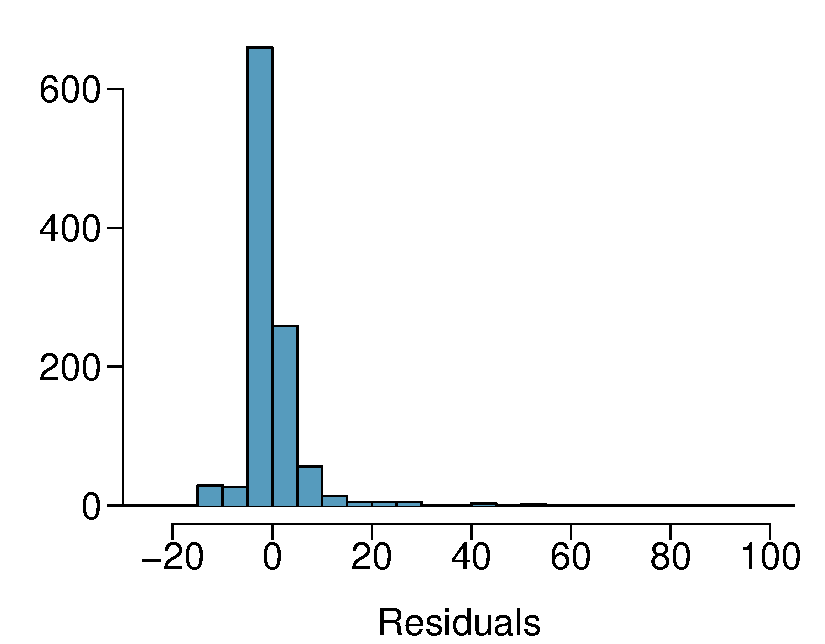
\includegraphics[width=0.47\textwidth]{ch_regr_mult_and_log/figures/eoce/movie_returns_altogether/horror_movies_conds_hist_res.pdf}\hspace{3mm}
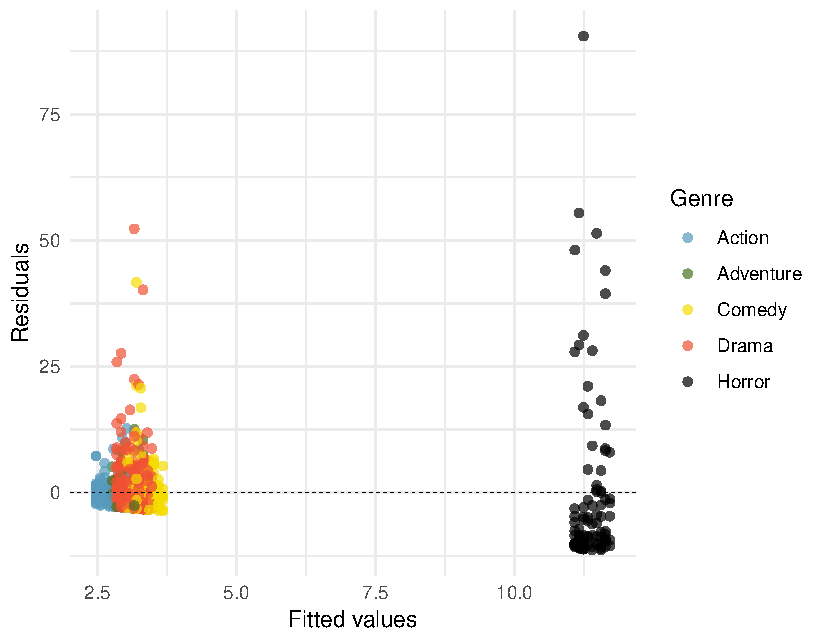
\includegraphics[width=0.47\textwidth]{ch_regr_mult_and_log/figures/eoce/movie_returns_altogether/horror_movies_conds_res_genre_fitted.pdf}\\[5mm]
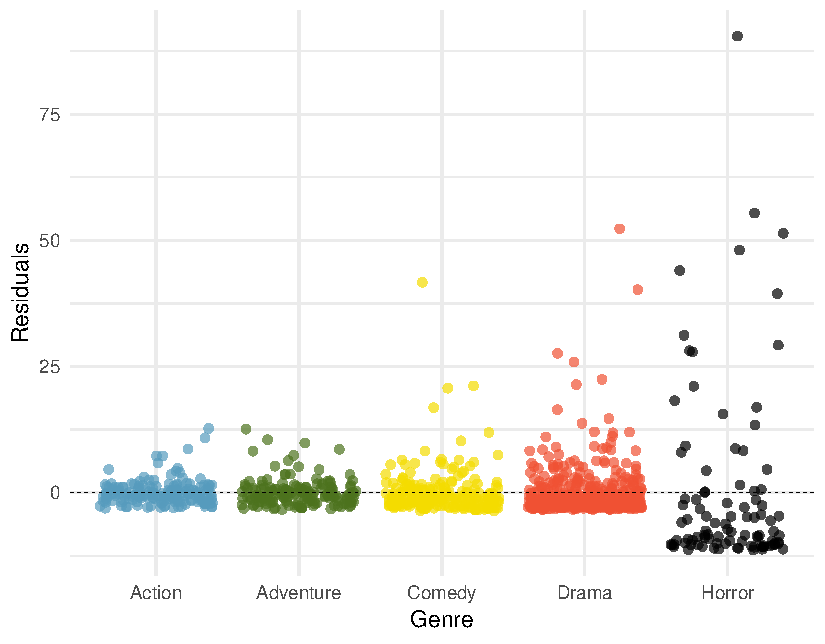
\includegraphics[width=0.47\textwidth]{ch_regr_mult_and_log/figures/eoce/movie_returns_altogether/horror_movies_conds_res_genre.pdf}\hspace{3mm}
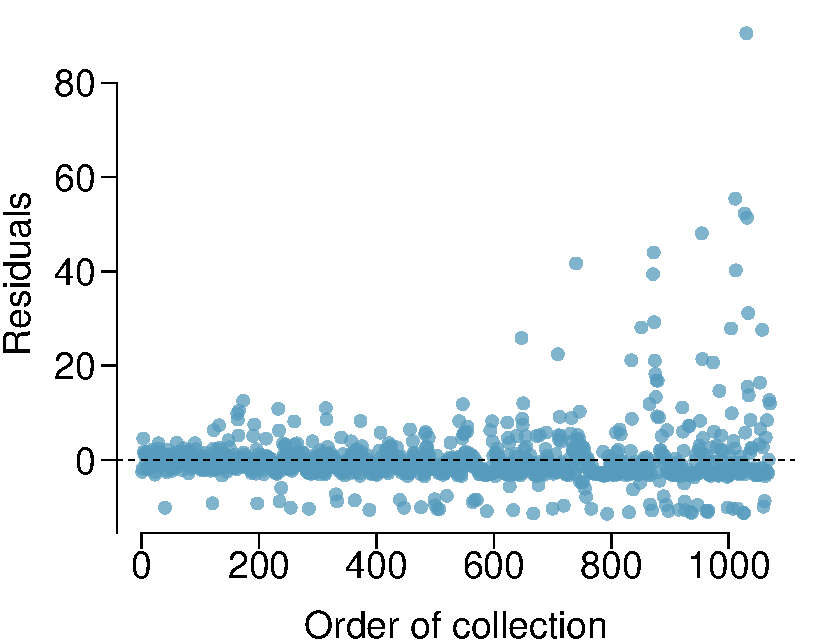
\includegraphics[width=0.47\textwidth]{ch_regr_mult_and_log/figures/eoce/movie_returns_altogether/horror_movies_conds_res_order.pdf}\\[5mm]
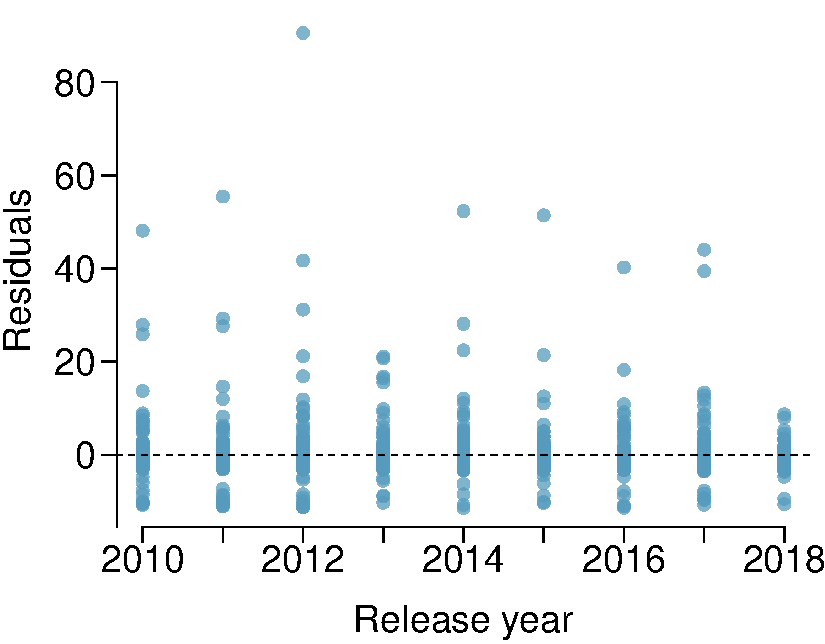
\includegraphics[width=0.47\textwidth]{ch_regr_mult_and_log/figures/eoce/movie_returns_altogether/horror_movies_conds_res_year.pdf} 
\end{center}
}{}
}






%_____________________
\section{Multiple regression case study: Mario Kart}
\label{mario_kart_case_study}

\noindent%
We'll consider Ebay auctions of a video game called
\emph{Mario Kart} for the Nintendo Wii.
The outcome variable of interest is the total price of
an auction, which is the highest bid plus the shipping cost.
We will try to determine how total price is related to each
characteristic in an auction while simultaneously controlling
for other variables.
For instance, all other characteristics held constant,
are longer auctions associated with higher or lower prices?
And, on average, how much more do buyers tend to pay for
additional Wii wheels
(plastic steering wheels that attach to the Wii controller)
in auctions?
Multiple regression will help us answer these and other questions.

\newcommand{\mknum}{141}


\subsection{Data set and the full model}

The \data{mariokart} data set includes results
from \mknum{}~auctions.
Four observations from this data set are shown in
Figure~\ref{marioKartDataMatrix},
and descriptions for each variable are shown in
Figure~\ref{marioKartVariables}. 
Notice that the condition and stock photo variables
are indicator variables\index{indicator variable},
similar to \var{bankruptcy} in the \data{loan} data set.
%For instance, the \var{cond\us{}new} variable takes value 1 if the game up for auction is new and 0 if it is used. Using indicator variables in place of category names allows for these variables to be directly used in regression.

\begin{figure}[ht]
\centering
\begin{tabular}{rrrrlr}
  \hline
  & price & cond\us{}new & stock\us{}photo & duration & wheels \\ 
  \hline
  1 & 51.55 &   1 & 1 & 3 &   1 \\ 
  2 & 37.04 &  0 &  1 & 7 &   1 \\ 
  $\vdots$ &$\vdots$ &$\vdots$ &$\vdots$ &$\vdots$ &$\vdots$ \\
  140 & 38.76 &  0 &  0 & 7 &   0 \\ 
  141 & 54.51 &  1 &  1 & 1 &   2 \\ 
  \hline
\end{tabular}
\caption{Four observations from the \data{mariokart}
    data set.}
\label{marioKartDataMatrix}
\end{figure}
%library(openintro); data(marioKart); d <- marioKart[marioKart$totalPr < 100,]; row.names(d) <- NULL; d

\begin{figure}[h]
\centering\small
\begin{tabular}{lp{9.5cm}}
\hline
{\bf variable} & {\bf description} \\
\hline
\var{price} &
  Final auction price plus shipping costs, in US dollars. \\
\var{cond\us{}new} &
  Indicator variable for if the game is new (\resp{1}) or used (\resp{0}). \\
\var{stock\us{}photo} &
  Indicator variable for if the auction's main photo
  is a stock photo. \\
\var{duration} &
  The length of the auction, in days, taking values from 1 to 10. \\
\var{wheels} &
  The number of Wii wheels included with the auction.
  A \emph{Wii wheel} is an optional steering wheel accessory
  that holds the Wii controller. \\
\hline
\end{tabular}
\caption{Variables and their descriptions for the
    \data{mariokart} data set.}
\label{marioKartVariables}
\end{figure}

% library(openintro); library(xtable); data(marioKart); d <- marioKart[marioKart$totalPr < 100,]; d$cond <- relevel(d$cond, "used"); xtable(lm(d$totalPr ~ d$cond)); xtable(lm(d$totalPr ~ d$duration))

%\begin{figure}[h]
%  \centering
%  \Figure{0.5}{marioKartSingle}
%  \caption{Scatterplot of the total auction price against the
%      game's condition.
%      The least squares line is also shown.}
%  \label{marioKartSingle}
%\end{figure}

\D{\newpage}

\begin{exercisewrap}
\begin{nexercise}
\label{condNewVarForMarioKartOnly}
We fit a linear regression model with
the game's condition as a predictor of auction price.
Results of this model are summarized below:
\begin{center}
\begin{tabular}{rrrrr}
  \hline
  \vspace{-3.7mm} & & & & \\
 & Estimate & Std. Error & t value & Pr($>$$|$t$|$) \\ 
  \hline
  \vspace{-3.8mm} & & & & \\
(Intercept) & 42.8711 & 0.8140 & 52.67 & $<$0.0001 \\ 
  cond\us{}new & 10.8996 & 1.2583 & 8.66 & $<$0.0001 \\ 
   \hline
   &&&\multicolumn{2}{r}{$df=139$}
\end{tabular}
\end{center}
Write down the equation for the model,
note whether the slope is statistically different from zero,
and interpret the coefficient.\footnotemark{}
\end{nexercise}
\end{exercisewrap}
\footnotetext{The equation for the line may be written as
  \begin{align*}
  \widehat{price}
      &= 42.87 + 10.90\times cond\us{}new
  \end{align*}
  Examining the regression output in
  Guided Practice~\ref{condNewVarForMarioKartOnly},
  we can see that the p-value for \var{cond\us{}new}
  is very close to zero, indicating there is strong evidence
  that the coefficient is different from zero when using this
  simple one-variable model.

  The \var{cond\us{}new} is a two-level
  categorical variable that takes value 1 when the game is new
  and value 0 when the game is used.
  This means the 10.90 model coefficient predicts an extra
  \$10.90 for those games that are new versus those that are used.}

Sometimes there are underlying structures or relationships between predictor variables. For instance, new games sold on Ebay tend to come with more Wii wheels, which may have led to higher prices for those auctions. We would like to fit a model that includes all potentially important variables simultaneously. This would help us evaluate the relationship between a predictor variable and the outcome while controlling for the potential influence of other variables.

We want to construct a model that accounts for not only the game
condition, as in Guided Practice~\ref{condNewVarForMarioKartOnly},
but simultaneously accounts for three other variables:
\begin{align*}
\widehat{\var{price}}
	&= \beta_0 + \beta_1\times \var{cond\us{}new} +
		\beta_2\times \var{stock\us{}photo} \\
	&\qquad\  + \beta_3 \times  \var{duration} +
		\beta_4 \times  \var{wheels}
\end{align*}
Figure~\ref{MarioKartFullModelOutput} summarizes the full model.
Using this output, we identify the point estimates of each
coefficient.

\begin{figure}[ht]
\centering
\begin{tabular}{rrrrr}
  \hline
  \vspace{-3.7mm} & & & & \\
 & Estimate & Std. Error & t value & Pr($>$$|$t$|$) \\ 
  \hline
  \vspace{-3.8mm} & & & & \\
(Intercept) & 36.2110 & 1.5140 & 23.92 & $<$0.0001 \\ 
  cond\us{}new & 5.1306 & 1.0511 & 4.88 & $<$0.0001 \\ 
  stock\us{}photo & 1.0803 & 1.0568 & 1.02 & 0.3085 \\ 
  duration & -0.0268 & 0.1904 & -0.14 & 0.8882 \\ 
  wheels & 7.2852 & 0.5547 & 13.13 & $<$0.0001 \\ 
   \hline
   &&&\multicolumn{2}{r}{$df=136$}
\end{tabular}
\caption{Output for the regression model where \var{price} is the outcome and \var{cond\us{}new}, \var{stock\us{}photo}, \var{duration}, and \var{wheels} are the predictors.}
\label{MarioKartFullModelOutput}
\end{figure}
%library(openintro); library(xtable); data(marioKart); d <- marioKart[marioKart$totalPr < 100,]; d$cond <- relevel(d$cond, "used"); g <-lm(totalPr ~ cond + stockPhoto + duration + wheels, d)

\begin{exercisewrap}
\begin{nexercise}
\label{eqForMultRegrOfTotalPrForAllPredWithCoef}%
Write out the model's equation using the point estimates from
Figure~\ref{MarioKartFullModelOutput}.
How many predictors are there in this model?\footnotemark{}
\end{nexercise}
\end{exercisewrap}
\footnotetext{$\widehat{price}
    = 36.21
        + 5.13 \times \var{cond\us{}new}
        + 1.08 \times \var{stock\us{}photo}
        - 0.03 \times \var{duration}
        + 7.29 \times \var{wheels}$,
  with the $k=4$ predictors.}

\begin{exercisewrap}
\begin{nexercise}
What does $\beta_4$, the coefficient of variable
$x_4$ (Wii wheels), represent?
What is the point estimate of $\beta_4$?\footnotemark{}
\end{nexercise}
\end{exercisewrap}
\footnotetext{It is the average difference in auction price
  for each additional Wii wheel included when holding the
  other variables constant.
  The point estimate is $b_4 = 7.29$.}

\begin{exercisewrap}
\begin{nexercise}
\label{computeMultipleRegressionResidualForMarioKart}%
Compute the residual of the first observation in
Figure~\ref{marioKartDataMatrix} using the equation identified
in Guided Practice~\ref{eqForMultRegrOfTotalPrForAllPredWithCoef}.%
\footnotemark{}
\end{nexercise}
\end{exercisewrap}
\footnotetext{$e_i = y_i - \hat{y_i} = 51.55 - 49.62 = 1.93$,
  where 49.62 was computed using the variables values from the
  observation and the equation identified in
  Guided Practice~\ref{eqForMultRegrOfTotalPrForAllPredWithCoef}.}

\begin{examplewrap}
\begin{nexample}{We estimated a coefficient for
    \var{cond\us{}new} in
    Section~\ref{condNewVarForMarioKartOnly}
    of $b_1 = 10.90$ with a standard error of $SE_{b_1} = 1.26$
    when using simple linear regression.
    Why might there be a difference between that estimate
    and the one in the multiple regression setting?}
  \label{colinearityOfCondNewAndStockPhoto}%
  If we examined the data carefully, we would see that
  there is collinearity\index{collinear} among some predictors.
  For instance, when we estimated the connection of the outcome
  \var{price} and predictor \var{cond\us{}new} using simple linear
  regression, we were unable to control for other variables like
  the number of Wii wheels included in the auction.
  That model was biased by the confounding variable \var{wheels}.
  When we use both variables, this particular underlying and
  unintentional bias is reduced or eliminated (though bias
  from other confounding variables may still remain).
\end{nexample}
\end{examplewrap}


\subsection{Model selection}

\noindent%
Let's revisit the model for the Mario Kart auction and complete
model selection using backwards selection.
Recall that the full model took the following form:
\begin{align*}
\widehat{price} = 36.21
    + 5.13 \times \var{cond\us{}new}
    + 1.08 \times \var{stock\us{}photo}
    - 0.03 \times \var{duration}
    + 7.29 \times \var{wheels}
\end{align*}


\begin{examplewrap}
\begin{nexample}{Results corresponding to the full model
    for the \data{mariokart} data were shown
    in Figure~\vref{MarioKartFullModelOutput}.
    For this model, we consider what would happen if dropping
    each of the variables in the model:
    \begin{center}
    \begin{tabular}{lllll}
    Exclude ... &
      \var{cond\us{}new} &
      \var{stock\us{}photo} &
      \var{duration} &
      \var{wheels} \\
    &
      $R^2_{adj} = 0.6626$ &
      $R^2_{adj} = 0.7107$ &
      $R^2_{adj} = 0.7128$ &
      $R^2_{adj} = 0.3487$ \\
    \end{tabular}
    \end{center}
    For the full model, $R_{adj}^2 = 0.7108$.
    How should we proceed under the backward elimination strategy?}
  \label{backwardEliminationExampleWMarioKartData}%
  The third model without \var{duration} has the highest
  $R_{adj}^2$ of 0.7128, so we compare it to
  $R_{adj}^2$ for the full model.
  Because eliminating \var{duration} leads to a model with
  a higher $R_{adj}^2$, we drop \var{duration} from the model.
\end{nexample}
\end{examplewrap}

\begin{exercisewrap}
\begin{nexercise}
In Example~\ref{backwardEliminationExampleWMarioKartData},
we eliminated the \var{duration} variable,
which resulted in a model with $R_{adj}^2 = 0.7128$.
Let's look at if we would eliminate another variable from the
model using backwards elimination:
\begin{center}
\begin{tabular}{llll}
Exclude \var{duration} and ... &
	\var{cond\us{}new} &
	\var{stock\us{}photo} &
	\var{wheels} \\
&
	$R^2_{adj} = 0.6587$ &
	$R^2_{adj} = 0.7124$ &
	$R^2_{adj} = 0.3414$ \\
\end{tabular}
\end{center}
Should we eliminate any additional variable, and if so,
which variable should we eliminate?\footnotemark{}
\end{nexercise}
\end{exercisewrap}
\footnotetext{Removing any of the three remaining variables
  would lead to a decrease in $R_{adj}^2$, so we should not
  remove any additional variables from the model after we
  removed \var{duration}.}

\D{\newpage}

\begin{exercisewrap}
\begin{nexercise}
\label{totPrPredictionUsedStockPhotoTwoWheels}%
After eliminating the auction's duration from the model,
we are left with the following reduced model:
\begin{align*}
\widehat{price} &= \ 36.05
    + 5.18 \times \text{\var{cond\us{}new}}
    + 1.12 \times \text{\var{stock\us{}photo}}
    + 7.30 \times \text{\var{wheels}}
\end{align*}
How much would you predict for the total price for
the Mario Kart game if it was used, used a stock photo,
and included two wheels and put up for auction during
the time period that the Mario Kart data were
collected?\footnotemark{}
\end{nexercise}
\end{exercisewrap}
\footnotetext{We would plug in \resp{0} for \var{cond\us{}new}
  \resp{1} for \var{stock\us{}photo},
  and \resp{2} for \var{wheels} into the equation,
  which would return \$51.77, which is the total price
  we would expect for the auction.}

\begin{exercisewrap}
\begin{nexercise}
Would you be surprised if the seller from
Guided Practice~\ref{totPrPredictionUsedStockPhotoTwoWheels}
didn't get the exact price predicted?\footnotemark{}
\end{nexercise}
\end{exercisewrap}
\footnotetext{No.
  The model provides the \emph{average} auction price
  we would expect, and the price for one auction to the next
  will continue to vary a bit
  (but less than what our prediction would be without the model).}

%If we continued the process, we would not eliminate any additional  of these models lead to an improvement in adjusted $R^2$, so we do not eliminate any of the remaining predictors. That is, after backward elimination, we are left with the model that keeps \var{cond\us{}new}, \var{stock\us{}photos}, and \var{wheels}, which we can summarize using the coefficients from Table~\ref{marioKartMultipleRegressionModelAllButDuration}:
%\begin{align*}
%\hat{y} \ &= \ b_0 + b_1x_1 + b_2x_2 + b_4x_4 \\
%\widehat{price} &= \ 36.05 + 5.18 \times \text{\var{cond\us{}new}} + 1.12 \times \text{\var{stock\us{}photo}} + 7.30 \times \text{\var{wheels}}
%\end{align*}


\subsection{Checking model conditions using graphs}

\noindent%
Let's take a closer look at the diagnostics for the Mario Kart
model to check if the model we have identified is reasonable.

\begin{description}
\item[Check for outliers.]
    A histogram of the residuals is shown in
    Figure~\ref{mkDiagResHist}.
    With a data set well over a hundred, we're primarily
    looking for major outliers.
    While one minor outlier appears on the upper end,
    it is not a concern for this large of a data set.

\begin{figure}[h]
  \centering
  \Figures{0.6}{marioKartDiagnostics}
      {mkDiagResHist}
  \caption{Histogram of the residuals.
      No clear outliers are evident.}
  \label{mkDiagResHist}
\end{figure}

\item[Absolute values of residuals against fitted values.]
    A plot of the absolute value of the residuals against
    their corresponding fitted values ($\hat{y}_i$) is shown
    in Figure~\ref{mkDiagnosticEvsAbsF}.
    We don't see any obvious deviations from constant variance
    in this example.

\begin{figure}
  \centering
  \Figures{0.6}{marioKartDiagnostics}{mkDiagnosticEvsAbsF}
  \caption{Absolute value of the residuals against
      the fitted values.
      No patterns are evident.}
  \label{mkDiagnosticEvsAbsF}
\end{figure}

\item[Residuals in order of their data collection.]
    A plot of the residuals in the order their corresponding
    auctions were observed is shown in
    Figure~\ref{mkDiagnosticInOrder}.
    Here we see no structure that indicates a problem.

\begin{figure}[h]
  \centering
  \Figures{0.55}{marioKartDiagnostics}{mkDiagnosticInOrder}
  \caption{Residuals in the order that their
      corresponding observations were collected.
      There are no evident patterns.}
  \label{mkDiagnosticInOrder}
\end{figure}

\item[Residuals against each predictor variable.]
    We consider a plot of the residuals against the
    \var{cond\us{}new} variable, the residuals against
    the \var{stock\us{}photo} variable,
    and the residuals against the \var{wheels} variable.
    These plots are shown in Figure~\ref{mkDiagnosticEvsVariables}.
    For the two-level condition variable, we are guaranteed not
    to see any remaining trend, and instead we are checking that
    the variability doesn't fluctuate across groups,
    which it does not.
    However, looking at the stock photo variable,
    we find that there is some difference in the variability
    of the residuals in the two groups.
    Additionally, when we consider the residuals against the
    \var{wheels} variable, we see some possible structure.
    There appears to be curvature in the residuals,
    indicating the relationship is probably not linear.

\begin{figure}
  \centering
  \Figures{0.9}{marioKartDiagnostics}{mkDiagnosticEvsVariables}
  \caption{For the condition and stock photo variables,
      we check
      for differences in the distribution shape
      or variability of
      the residuals.
      In the case of the stock photos variable,
      we see a little
      less variability in the unique photo group
      than the stock
      photo group.
      For numerical predictors, we also check for
      trends or other structure.
      We see some slight bowing in the residuals against the
      \var{wheels} variable in the bottom plot.}
  \label{mkDiagnosticEvsVariables}
\end{figure}

\end{description}

As with the \data{loans} analysis, we would summarize
diagnostics when reporting the model results.
In the case of this auction data,
we would report that there appears to be non-constant variance
in the stock photo variable and that there may be a nonlinear
relationship between the total price and the number of wheels
included for an auction.
This information would be important to buyers and sellers who
may review the analysis, and omitting this information could be
a setback to the very people who the model might assist. \\

\noindent%
\textbf{Note: there are no exercises for this section.}




%__________________
\section{Introduction to logistic regression}
\label{logisticRegression}

\index{logistic regression|seealso{regression}}
\index{regression!logistic|(}

\noindent%
In this section we introduce
\termsub{logistic regression}{regression!logistic}
as a tool for building models when there is a categorical
response variable with two levels, e.g. yes and no.
Logistic regression is a type of
\term{generalized linear model} (\term{GLM})
for response variables
where regular multiple regression does not work very well.
In particular, the response variable in these settings often
takes a form where residuals look completely different from
the normal distribution.

GLMs can be thought of as a two-stage modeling approach.
We first model the response variable using a probability
distribution, such as the binomial or Poisson distribution.
Second, we model the parameter of the distribution using
a collection of predictors and a special form of multiple
regression.
Ultimately, the application of a GLM will feel very similar
to multiple regression, even if some of the details are
different.

%In Section~\ref{logisticRegression} we will revisit the \data{email} data set from Chapter~\ref{introductionToData}. These emails were collected from a single email account, and we will work on developing a basic spam filter using these data. The response variable, \var{spam}, has been encoded to take value~0 when a message is not spam and~1 when it is spam. Our task will be to build an appropriate model that classifies messages as spam or not spam using email characteristics coded as predictor variables. While this model will not be the same as those used in large-scale spam filters, it shares many of the same features. 

\subsection{Resume data}

\index{data!resume|(}

\newcommand{\resN}{4870}
\newcommand{\resCallbackProp}{0.0805}
\newcommand{\resCallbackPerc}{8.05\%}
\newcommand{\resNumPred}{8}
\newcommand{\resUniqueNames}{36}
\newcommand{\resHonorsInt}{-2.4998}
\newcommand{\resHonorsCoef}{0.8668}
\newcommand{\resHonorsIntPlusCoef}{-1.6330}
\newcommand{\resHonorsCoefSE}{0.1776}
\newcommand{\resHonorsCoefZ}{4.88}
\newcommand{\resHonorsProb}{0.163}
\newcommand{\resHonorsPerc}{16.3\%}
\newcommand{\resHonorsNotProb}{0.076}
\newcommand{\resHonorsNotPerc}{7.6\%}

We will consider experiment data from a study that sought
to understand the effect of race and sex on job application
callback rates;
details of the study and a link to the data set may be
found in Appendix~\ref{ch_regr_mult_and_log_data}.
To evaluate which factors were important,
job postings were identified in Boston and Chicago
for the study,
and researchers created many fake resumes to send off
to these jobs to see which would elicit a callback.
The researchers enumerated important characteristics,
such as years of
experience and education details, and they used these
characteristics to randomly generate the resumes.
Finally, they randomly assigned a name to each resume,
where the name would imply the applicant's sex and race.

The first names that were used and randomly assigned
in this experiment were selected so that they
would predominantly be recognized as belonging
to Black or White individuals;
other races were not considered in this study.
While no name would definitively be inferred as pertaining
to a Black individual or to a White individual,
the researchers conducted a survey to check for
racial association of the names;
names that did not pass this survey check were excluded
from usage in the experiment.
You can find the full set of names that did pass the
survey test and were ultimately used in the study in
Figure~\ref{resumeFirstName}.
For example, Lakisha was a name that their survey indicated
would be interpreted as a Black woman, while Greg was a name
that would generally be interpreted to be associated with
a White male.

\begin{figure}[h]
\centering\small
\begin{tabular}{lll c lll c lll}
  \cline{1-3} \cline{5-7} \cline{9-11}
  first\us{}name & race & sex
      & \ \hspace{2mm}\ &
      first\us{}name & race & sex
      & \ \hspace{2mm}\ &
      first\us{}name & race & sex
      \\
  \cline{1-3} \cline{5-7} \cline{9-11}
  Aisha & black & female &&
      Hakim & black & male &&
      Laurie & white & female \\
  Allison & white & female &&
      Jamal & black & male &&
      Leroy & black & male \\
  Anne & white & female &&
      Jay & white & male &&
      Matthew & white & male \\
  Brad & white & male &&
      Jermaine & black & male &&
      Meredith & white & female \\
  Brendan & white & male &&
      Jill & white & female &&
      Neil & white & male \\
  Brett & white & male &&
      Kareem & black & male &&
      Rasheed & black & male \\
  Carrie & white & female &&
      Keisha & black & female &&
      Sarah & white & female \\
  Darnell & black & male &&
      Kenya & black & female &&
      Tamika & black & female \\
  Ebony & black & female &&
      Kristen & white & female &&
      Tanisha & black & female \\
  Emily & white & female &&
      Lakisha & black & female &&
      Todd & white & male \\
  Geoffrey & white & male &&
      Latonya & black & female &&
      Tremayne & black & male \\
  Greg & white & male &&
      Latoya & black & female &&
      Tyrone & black & male \\
  \cline{1-3} \cline{5-7} \cline{9-11}
\end{tabular}
\caption{List of all \resUniqueNames{} unique names along
    with the commonly inferred race and sex associated
    with these names.}
\label{resumeFirstName}
\end{figure}
% library(openintro); library(xtable); vars <- c("firstname", "race", "gender"); d <- resume[, vars]; names(d)[1] <- "first_name"; d <- unique(d); d <- d[order(d$first_name), ]; rownames(d) <- NULL; d. <- cbind(d[1:12, ], d[13:24, ], d[25:36, ]); xtable(d.)

The response variable of interest is whether or not there
was a callback from the employer for the applicant,
and there were \resNumPred{} attributes that
were randomly assigned that we'll consider,
with special interest in the race and sex variables.
Race and sex are \term{protected classes} in the
United States, meaning they are not legally permitted
factors for hiring or employment decisions.
The full set of attributes considered is provided in
Figure~\ref{resumeVariables}.

\D{\newpage}

\begin{figure}[h]
\centering\small
\begin{tabular}{lp{112mm}}
\hline
{\bf variable} & {\bf description} \\
\hline
\var{callback} &
    Specifies whether the employer called the applicant
    following submission of the application for the job. \\
%\var{first\us{}name} &
%    First name of the applicant that is listed on the resume. \\
\var{job\us{}city} &
    City where the job was located: Boston or Chicago.\\
%\var{job\us{}industry} &
%    The job industry, e.g. manufacturing or transportation,
%    for the job listing. \\
%\var{job\us{}type} &
%    The type of job, e.g. supervisor or sales representative,
%    for the job listing. \\
%\var{job\us{}req} &
%    An indicator for if there were any job requirements listed
%    in the job listing. \\
\var{college\us{}degree} &
    An indicator for whether the resume listed a college degree. \\
\var{years\us{}experience} &
    Number of years of experience listed on the resume. \\
\var{honors} &
    Indicator for the resume listing some sort of honors,
    e.g.~employee of the month. \\
\var{military} &
    Indicator for if the resume listed any military experience. \\
\var{email\us{}address} &
    Indicator for if the resume listed an email address for
    the applicant. \\
\var{race} &
    Race of the applicant, implied by their first name
    listed on the resume. \\
\var{sex} &
    Sex of the applicant (limited to only \resp{male}
    and \resp{female} in this study),
    implied by the first name listed on the resume. \\
\hline
\end{tabular}
\caption{Descriptions for the \var{callback} variable
    along with \resNumPred{} other variables
    in the \data{resume} data set.
    Many of the variables are
    indicator\index{indicator variable} variables,
    meaning they take the value 1 if the specified
    characteristic is present and 0 otherwise.}
\label{resumeVariables}
\end{figure}

All of the attributes listed on each resume were
randomly assigned.
This means that no attributes that might be favorable
or detrimental to employment would favor one demographic
over another on these resumes.
Importantly, due to the experimental nature of this study,
we can infer causation between these variables and the
callback rate, if the variable is statistically significant.
Our analysis will allow us to compare the practical
importance of each of the variables relative to each other.




\subsection{Modeling the probability of an event}
\label{modelingTheProbabilityOfAnEvent}

Logistic regression is a generalized linear model where
the outcome is a two-level categorical variable.
The outcome, $Y_i$, takes the value 1
(in our application, this represents a callback
for the resume)
with probability $p_i$
and the value 0 with probability $1 - p_i$.
Because each observation has a slightly different
context, e.g. different education level or a different
number of years of experience, the probability $p_i$
will differ for each observation.
Ultimately, it is this probability that we model
in relation to the predictor variables:
we will examine which resume characteristics
correspond to higher or lower callback rates.

\begin{onebox}{Notation for a logistic regression model}
The outcome variable for a GLM is denoted by $Y_i$,
where the index $i$ is used to represent observation $i$.
In the resume application, $Y_i$ will be used to represent
whether resume $i$ received a callback ($Y_i=1$)
or not ($Y_i=0$). \vspace{3mm}

The predictor variables are represented as follows:
$x_{1,i}$ is the value of variable 1 for observation $i$,
$x_{2,i}$ is the value of variable 2 for observation $i$,
and so on.
\end{onebox}

The logistic regression model relates the probability
a resume would receive a callback ($p_i$) to the predictors
$x_{1,i}$, $x_{2,i}$, ..., $x_{k,i}$
through a framework much like that of multiple regression:
\begin{align}
transformation(p_{i})
  = \beta_0 +
      \beta_1x_{1,i} +
      \beta_2 x_{2,i} +
      \cdots +
      \beta_k x_{k,i}
\label{linkTransformationEquation}
\end{align}
We want to choose a transformation in the equation
that makes practical and mathematical sense.
For example, we want a transformation that makes
the range of possibilities on the left hand side
of the equation equal to the range of possibilities
for the right hand side;
if there was no transformation for this equation,
the left hand side could only take values between 0 and 1,
but the right hand side could take values outside of this
range.
A common transformation for $p_i$ is the \term{logit transformation}, which may be written as
\begin{align*}
logit(p_i) = \log_{e}\left( \frac{p_i}{1-p_i} \right)
\end{align*}
The logit transformation is shown in
Figure~\ref{logitTransformationFigureHoriz}.
Below, we rewrite the equation relating $Y_i$ to its
predictors using the logit transformation of $p_i$:
\begin{align*}
\log_{e}\left( \frac{p_i}{1-p_i} \right)
  = \beta_0 +
      \beta_1 x_{1,i} +
      \beta_2 x_{2,i} +
      \cdots +
      \beta_k x_{k,i}
\end{align*}
In our resume example, there are \resNumPred{} predictor
variables, so $k = \resNumPred{}$.
While the precise choice of a logit function isn't intuitive,
it is based on theory that underpins generalized linear models,
which is beyond the scope of this book.
Fortunately, once we fit a model using software,
it will start to feel like we're back in the
multiple regression context, even if the
interpretation of the coefficients is more complex.

\begin{figure}
  \centering
  \Figure{}{logitTransformationFigureHoriz}
  \caption{Values of $p_i$ against values of $logit(p_i)$.}
  \label{logitTransformationFigureHoriz}
\end{figure}

\begin{examplewrap}
\begin{nexample}{We start by fitting a model with a single
    predictor: \var{honors}.
    This variable indicates whether the applicant had any
    type of honors listed on their resume,
    such as employee of the month.
    The following logistic regression model was fit using
    statistical software:
    \begin{align*}
    \log\left( \frac{p_i}{1-p_i} \right)
      = \resHonorsInt{} +
          \resHonorsCoef{} \times\text{\var{honors}}
    \end{align*}
    %library(openintro); m <- glm(received_callback ~ honors, data = resume, family=binomial); summary(m); co <- round(m$coefficients, 4); a <- exp(co["(Intercept)"]); a/(1+a); a <- exp(sum(co)); a/(1+a)
    (a) If a resume is randomly selected from the study
    and it does not have any honors listed,
    what is the probability resulted in a callback?
    
    (b) What would the probability be if the resume did
    list some honors?}
    \label{logisticExampleWithHonors}%
  (a) If a randomly chosen resume from those sent out is considered,
  and it does not list honors, then \var{honors} takes
  value~0 and the right side of the model equation equals
  \resHonorsInt{}.
  Solving for $p_i$:
  $\frac{e^{\resHonorsInt{}}}{1 + e^{\resHonorsInt{}}}
      = \resHonorsNotProb{}$.
  Just as we labeled a fitted value of $y_i$ with a ``hat''
  in single-variable and multiple regression, we do the same
  for this probability: $\hat{p}_i = \resHonorsNotProb{}$.

  (b) If the resume had listed some honors,
  then the right side of the model equation is
  $\resHonorsInt{} + \resHonorsCoef{} \times 1
      = \resHonorsIntPlusCoef{}$,
  which corresponds to a probability
  $\hat{p}_i = \resHonorsProb{}$.

  Notice that we could examine \resHonorsInt{} and
  \resHonorsIntPlusCoef{} in
  Figure~\ref{logitTransformationFigureHoriz}
  to estimate the probability before formally calculating
  the value.
\end{nexample}
\end{examplewrap}

\D{\newpage}

To convert from values on the logistic regression scale
(e.g. \resHonorsInt{} and \resHonorsIntPlusCoef{} in
Example~\ref{logisticExampleWithHonors}),
use the following formula, which is the result
of solving for $p_i$ in the regression model:
\newcommand{\exponentialToSolveForPi}
    {e^{\beta_0 + \beta_1 x_{1,i}+\cdots+\beta_k x_{k,i}}}%
\begin{align*}
p_i = \frac{\exponentialToSolveForPi{}}
    {\ 1\ \ +\ \ \exponentialToSolveForPi{}\ }
\end{align*}
As with most applied data problems,
we substitute the point estimates for the parameters
(the $\beta_i$) so that we can make use of this formula.
In Example~\ref{logisticExampleWithHonors},
the probabilities were calculated as
\begin{align*}
&\frac{\ e^{\resHonorsInt{}}\ }
    {\ 1\ +\ e^{\resHonorsInt{}}\ }
  = \resHonorsNotProb{} &&
\frac{\ e^{\resHonorsInt{} + \resHonorsCoef{}}\ }
    {\ 1\ +\ e^{\resHonorsInt{} + \resHonorsCoef{}}\ }
  = \resHonorsProb{}
\end{align*}
While knowing whether a resume listed honors provides
some signal when predicting whether or not the employer
would call, we would like to account for many different
variables at once to understand how each of the different
resume characteristics affected the chance of a callback.


\subsection{Building the logistic model with many variables}

We used statistical software to fit the logistic regression
model with all \resNumPred{} predictors described in
Figure~\ref{resumeVariables}.
Like multiple regression, the result may be presented
in a summary table, which is shown in
Figure~\ref{resumeLogisticModelResults}.
The structure of this table is almost identical to that
of multiple regression;
the only notable difference is that the p-values are
calculated using the normal distribution rather than
the $t$-distribution.

\begin{figure}[ht]
\centering
\begin{tabular}{l rrrr}
  \hline
  \vspace{-3.7mm} & & & & \\
  & Estimate & Std. Error & z value & Pr($>$$|$z$|$) \\
  \hline
  \vspace{-3.8mm} & & & & \\
  (Intercept) & -2.6632 & 0.1820 & -14.64 & $<$0.0001 \\
  job\us{}city\lmlevel{Chicago} &
      -0.4403 & 0.1142 & -3.85 & 0.0001 \\
  college\us{}degree & -0.0666 & 0.1211 & -0.55 & 0.5821 \\
  years\us{}experience & 0.0200 & 0.0102 & 1.96 & 0.0503 \\
  honors & 0.7694 & 0.1858 & 4.14 & $<$0.0001 \\
  military & -0.3422 & 0.2157 & -1.59 & 0.1127 \\
  email\us{}address & 0.2183 & 0.1133 & 1.93 & 0.0541 \\
  race\lmlevel{white} & 0.4424 & 0.1080 & 4.10 & $<$0.0001 \\
  sex\lmlevel{male} & -0.1818 & 0.1376 & -1.32 & 0.1863 \\
  \hline
\end{tabular}
\caption{Summary table for the full logistic regression model
    for the resume callback example.}
\label{resumeLogisticModelResults}
\end{figure}
% library(openintro); library(dplyr); a <- resume; d <- data.frame(callback = a$received_callback, job_city = a$job_city, college_degree = a$college_degree, years_experience = a$years_experience, honors = a$honors, military = a$military, email_address = a$has_email_address, race = a$race, gender = ifelse(a$gender == "m", "male", "female"))
% job_industry = a$job_industry, job_type = a$job_type, 
% m <- glm(callback ~ job_city + college_degree + years_experience + honors + military + email_address + race + gender, data = d, family = binomial); summary(m); xtable(m)
\newcommand{\resRaceWhiteCoef}{0.4424}

Just like multiple regression, we could trim some variables
from the model.
Here we'll use a statistic called
\term{Akaike information criterion (AIC)},
which is an analog to how we used adjusted R-squared
in multiple regression,
and we look for models with a lower AIC
through a backward elimination strategy.
After using this criteria, the \var{college\us{}degree}
variable is eliminated, giving the smaller model summarized
in Figure~\ref{resumeLogisticReducedModel},
which is what we'll rely on for the remainder
of this section.
%\Comment{Do we want to discuss that one variable dropping out more?}

\begin{figure}[ht]
\centering
\begin{tabular}{l rrrr}
  \hline
  \vspace{-3.7mm} & & & & \\
  & Estimate & Std. Error & z value & Pr($>$$|$z$|$) \\ 
  \hline
  \vspace{-3.8mm} & & & & \\
  (Intercept) & -2.7162 & 0.1551 & -17.51 & $<$0.0001 \\ 
  job\us{}city\lmlevel{Chicago} &
      -0.4364 & 0.1141 & -3.83 & 0.0001 \\ 
  years\us{}experience & 0.0206 & 0.0102 & 2.02 & 0.0430 \\ 
  honors & 0.7634 & 0.1852 & 4.12 & $<$0.0001 \\ 
  military & -0.3443 & 0.2157 & -1.60 & 0.1105 \\ 
  email\us{}address & 0.2221 & 0.1130 & 1.97 & 0.0494 \\ 
  race\lmlevel{white} & 0.4429 & 0.1080 & 4.10 & $<$0.0001 \\ 
  sex\lmlevel{male} & -0.1959 & 0.1352 & -1.45 & 0.1473 \\ 
\hline
\end{tabular}
\caption{Summary table for the logistic regression model
    for the resume callback example, where variable selection
    has been performed using AIC.}
\label{resumeLogisticReducedModel}
\end{figure}
% # Run code for table above first
% % m. <- step(m); summary(m.); xtable(m.)
\newcommand{\resRaceWhiteCoefReduced}{0.4429}

\begin{examplewrap}
\begin{nexample}{The \var{race} variable had taken
    only two levels: \resp{black} and \resp{white}.
    Based on the model results, was race a meaningful
    factor for if a prospective employer would
    call back?}
  We see that the p-value for this coefficient is very
  small (very nearly zero), which implies that race
  played a statistically significant role in whether
  a candidate received a callback.
  Additionally, we see that the coefficient shown
  corresponds to the level of \resp{white},
  and it is positive.
  This positive coefficient reflects a positive gain
  in callback rate for resumes where the candidate's
  first name implied they were White.  
  The data provide very strong evidence of racism
  by prospective employers that favors resumes where the
  first name is typically interpreted to be White.
\end{nexample}
\end{examplewrap}

%We, the authors, found this conclusion saddening,
%though not surprising.
%It is also important to consider that this data only
%highlights one stage of racial bias in employment --
%when someone is trying to get hired --
%and it does not consider racial bias during employment.
%It does not scratch the surface of racial bias
%for individuals who are hired.

%\begin{examplewrap}
%\begin{nexample}{Compare the coefficient of t.
%    Why are the two estimated coefficients different?}
%  We earlier discussed how the implied race on the resume
%  was randomized and this variable is independent of
%  other predictors.
%  This means that the estimated effect will be virtually
%  unchanged even after we add or remove other variables
%  from the model.
%  This property is the product of thoughtful experiment
%  design by this study's researchers.
%\end{nexample}
%\end{examplewrap}

The coefficient of $\indfunc{race}{white}$ in the full model in
Figure~\ref{resumeLogisticModelResults},
is nearly identical to the model shown in
Figure~\ref{resumeLogisticReducedModel}.
The predictors in this experiment were thoughtfully
laid out so that the coefficient estimates would typically
not be much influenced by which other predictors were 
in the model,
which aligned with the motivation of the study to tease
out which effects were important to getting a callback.
In most observational data,
it's common for point estimates to change a little,
and sometimes a lot, depending on which other
variables are included in the model.
%Collinearity can also occur in experiments,
%but in this case the experiment was designed in such a way
%that collinearity it was not an issue.
%This might happen if predictor variables are correlated,
%where the inclusion of one of the variables can influence.
%\Comment{Revisit the end of this paragraph,
%  e.g. if removing the Ebay auction example.}
%We previously saw this in the Ebay auction example when
%we compared the coefficient of \var{cond\us{}new} in a
%single-variable model and the corresponding coefficient
%in the multiple regression model when including three
%additional variables (see
%Sections~\ref{ind_and_cat_vars_as_predictors}
%and~\ref{includingAndAssessingManyVariablesInAModel}).

\begin{examplewrap}
\begin{nexample}{Use the model summarized in
    Figure~\ref{resumeLogisticReducedModel}
    to estimate the probability
    of receiving a callback for a job in Chicago
    where the candidate lists 14 years experience,
    no honors,
    no military experience,
    includes an email address,
    and has a first name that implies they are a White male.}
  \label{exampleForResumeAndWhiteQuantified}%
  We can start by writing out the equation using the
  coefficients from the model, then we can
  add in the corresponding values of each variable for this
  individual:
  \begin{align*}
  &log\left(\frac{p}{1 - p}\right) \\
    &\quad= - 2.7162
        - 0.4364 \times \indfunc{job\us{}city}{Chicago}
        + 0.0206 \times \var{years\us{}experience}
        + 0.7634 \times \var{honors} \\
      &\quad\qquad
          - 0.3443 \times \var{military}
          + 0.2221 \times \var{email}
          + 0.4429 \times \indfunc{race}{white}
          - 0.1959 \times \indfunc{sex}{male} \\
    &\quad= - 2.7162
        - 0.4364 \times 1
        + 0.0206 \times 14
        + 0.7634 \times 0 \\
      &\quad\qquad
          - 0.3443 \times 0
          + 0.2221 \times 1
          + 0.4429 \times 1
          - 0.1959 \times 1 \\
    &\quad= - 2.3955
  \end{align*}
  We can now back-solve for $p$:
  the chance such an individual will receive
  a callback is about~8.35\%.
\end{nexample}
\end{examplewrap}

\begin{examplewrap}
\begin{nexample}{Compute the probability of a callback
    for an individual with a name commonly inferred
    to be from a Black male but who otherwise
    has the same characteristics as the one described
    in Example~\ref{exampleForResumeAndWhiteQuantified}.}
  \index{exampleForResumeAndBlackQuantified}%
  We can complete the same steps for an individual
  with the same characteristics who is Black,
  where the only difference in the calculation is that
  the indicator variable
  $\indfunc{race}{white}$ will take a value of \resp{0}.
  Doing so yields a probability of 0.0553.
  Let's compare the results with those of
  Example~\ref{exampleForResumeAndWhiteQuantified}.

  In practical terms, an individual perceived
  as White based on their first name would need to
  apply to $\frac{1}{0.0835} \approx 12$ jobs on average
  to receive a callback,
  while an individual perceived as Black
  based on their first name
  would need
  to apply to $\frac{1}{0.0553} \approx 18$ jobs on average
  to receive a callback.
  That is, applicants who are perceived as
  Black need to apply to 50\% more employers
  to receive a callback than someone who is perceived
  as White based on their first name for jobs like
  those in the study.
\end{nexample}
\end{examplewrap}

What we've quantified in this section is alarming and disturbing.
However, one aspect that makes this racism so difficult to
address is that the experiment, as well-designed as it is,
cannot send us much signal about which employers are
discriminating.
It is only possible to say that discrimination is happening,
even if we cannot say which particular callbacks
-- or non-callbacks -- represent discrimination.
Finding strong evidence of racism for individual cases is
a persistent challenge in enforcing anti-discrimination laws.
%For observational data on racial discrimination,
%there are even more challenges:
%some variables may be correlated with race
%or there may be potential confounding variables that
%cannot reasonably be modeled,
%making the challenges even more profound in reliably
%identifying racism.



\subsection{Diagnostics for the callback rate model}
\label{logistic_regr_diagnostics_subsection}

\begin{onebox}{Logistic regression conditions}
There are two key conditions for fitting a logistic regression model:\vspace{-1mm}
\begin{enumerate}
\setlength{\itemsep}{0mm}
\item
    Each outcome $Y_i$ is independent of the other outcomes.
\item
    Each predictor $x_i$ is linearly related to logit$(p_i)$
    if all other predictors are held constant.
\end{enumerate}
\end{onebox}

The first logistic regression model condition
-- independence of the outcomes --
is reasonable for the experiment since characteristics
of resumes were randomly assigned to the resumes that
were sent out.
%This is further discussed in Appendix~\ref{}.

The second condition of the logistic regression model is
not easily checked without a fairly sizable amount of data.
Luckily, we have \resN{} resume submissions in the data set!
Let's first visualize these data by plotting the true
classification of the resumes against the model's fitted
probabilities, as shown in
Figure~\ref{logisticModelPredict}.
%The vast majority of emails (spam or not) still have fitted probabilities below 0.5.

\begin{figure}[h]
  \centering
  \Figures{0.95}{logisticModel}{logisticModelPredict}
  \caption{The predicted probability that each of the
      \resN{} resumes results in a callback.
      \hiddenterm{Noise}
      (small, random vertical shifts) have been added
      to each point so points with nearly identical
      values aren't plotted exactly on top of one another.}
  \label{logisticModelPredict}
\end{figure}

\D{\newpage}

%The probabilities predicted by the model fall between
%4.3\% and 29.9\%.
We'd like to assess the quality of the model.
For example, we might ask:
if we look at resumes that we modeled as having
a 10\% chance of getting a callback, do we find
about 10\% of them actually receive a callback?
We can check this for groups of the data by constructing
a plot as follows:
\begin{enumerate}
\item
    Bucket the data into groups based on their
    predicted probabilities.
\item
    Compute the average predicted probability for each group.
\item
    Compute the observed probability for each group,
    along with a 95\% confidence interval.
\item
    Plot the observed probabilities
    (with 95\% confidence intervals)
    against the average predicted probabilities for each group.
\end{enumerate}
The points plotted should fall close to the line $y = x$,
since the predicted probabilities should be similar to the
observed probabilities.
We can use the confidence intervals to roughly gauge whether
anything might be amiss.
Such a plot is shown in Figure~\ref{logisticModelBucketDiag}.

%To help us out, we'll borrow an advanced statistical
%method called \term{natural splines} that estimates
%the local probability over the region 0.04 to 0.30,
%which is the range of the predicted probabilities.
%All you need to know about natural splines to understand
%what we are doing is that they are used to fit flexible
%lines rather than straight lines.
%
%The curve fit using natural splines is shown in
%Figure~\ref{logisticModelSpline} as a solid black line.
%If the logistic model fits well, the curve should closely
%follow the dashed $y = x$ line.
%We have added shading to represent the confidence bound for
%the curved line to clarify what fluctuations might plausibly
%be due to chance.
%The dashed line generally stays within the error bound
%of the solid curve, suggesting the fit is reasonable.

\begin{figure}
  \centering
  \Figures{0.95}{logisticModel}{logisticModelBucketDiag}
      %{logisticModelSpline}
  \caption{The dashed line is within the confidence bound
       of the 95\% confidence intervals of each of the buckets,
       suggesting the logistic fit is reasonable.}
%  \caption{The dashed line is within the confidence bound
%       of the smoothed line, suggesting the logistic fit is
%       reasonable.}
  \label{logisticModelBucketDiag}
  %\label{logisticModelSpline}
\end{figure}

Additional diagnostics may be created that are similar to those
featured in Section~\ref{multipleRegressionModelAssumptions}.
For instance, we could compute residuals as
the observed outcome minus the expected outcome
($e_i = Y_i - \hat{p}_i$),
and then we could create plots of these residuals
against each predictor.
We might also create a plot like that in
Figure~\ref{logisticModelBucketDiag}
to better understand the deviations.
%We might also create a smoothed average like that in
%Figure~\ref{logisticModelSpline} to better understand
%deviations.

\index{data!resume|)}
\index{regression!logistic|)}
\index{regression|)}


\D{\newpage}

\subsection{Exploring discrimination between groups
    of different sizes}
    % An exercise in critical thinking around a hypothetical setting

\index{discrimination|(}

%Discrimination is an incredibly important and complex societal issue, and this study only examined discrimination in a single aspect
Any form of discrimination is concerning,
and this is why we decided it was so important to discuss
this topic using data.
The resume study also only examined discrimination in a
single aspect: whether a prospective employer would
call a candidate who submitted their resume.
There was a 50\% higher barrier for resumes simply when
the candidate had a first name that was perceived to be
from a Black individual.
It's unlikely that discrimination would stop there.

%Of course, discrimination can happen to anyone.
%Yet, discrimination against dominant groups is
%considered to be much less impactful than
%the discrimination experienced by oppressed groups.
%\emph{Why?}

\begin{examplewrap}
\begin{nexample}{Let's consider a sex-imbalanced
    company that consists of 20\% women
    and 80\% men,\footnotemark{}
    and we'll suppose that the
    company is very large, consisting of perhaps
    20,000 employees.
    Suppose when someone goes up for promotion at this
    company, 5~of their colleagues are randomly chosen
    to provide feedback on their work.
    \exspace{}

    Now let's imagine that 10\% of the people in the
    company are prejudiced against the other sex.
    That~is, 10\% of men are prejudiced against women,
    and similarly, 10\% of women are prejudiced against men.
    \exspace{}
    
    Who is discriminated against more at the company,
    men or women?}
  \label{sex_imbalance_leads_to_discrimination}%
  Let's suppose we took 100 men who have gone up for
  promotion in the past few years.
  For these men, $5 \times 100 = 500$ random colleagues
  will be tapped for their feedback, of which
  about 20\% will be women (100 women).
  Of these 100 women, 10 are expected to be biased
  against the man they are reviewing.
  Then, of the 500 colleagues reviewing them,
  men will experience
  discrimination by about 2\% of their colleagues when
  they go up for promotion.

  Let's do a similar calculation for 100 women
  who have gone up for promotion in the last few years.
  They will also have 500 random colleagues providing
  feedback, of which about 400 (80\%) will be men.
  Of these 400 men, about 40 (10\%) hold a bias against
  women.
  Of the 500 colleagues providing feedback on the
  promotion packet for these women, 8\% of the
  colleagues hold a bias against the women.
\end{nexample}
\end{examplewrap}
\footnotetext{A more thoughtful example would include
    non-binary individuals.}

Example~\ref{sex_imbalance_leads_to_discrimination}
highlights something profound:
even in a hypothetical setting where each demographic
has the same degree of prejudice
against the other demographic, the smaller group
experiences the negative effects more frequently.
Additionally, if we would complete a handful of examples
like the one above with different numbers,
we'd learn that the greater the imbalance
in the population groups, the more the smaller group
is disproportionately impacted.\footnote{%
  If a proportion $p$ of a company are
  women and the rest of the company consists of men,
  then under the hypothetical situation
  the ratio of rates of discrimination against women
  vs men would be given by $\frac{1 - p}{p}$;
  this ratio is always greater than 1 when $p < 0.5$.}%
%That is, this mathematical property may lead
%to more discrimination against a minority group,
%and the degree of that discrimination
%will be larger the greater the imbalance in the
%population under the scenario described.

Of course, there are other considerable real-world omissions
from the hypothetical example.
For example, studies have found instances where people from an
oppressed group also discriminate against others within their
own oppressed group.
As another example,
there are also instances where a majority group
can be oppressed, with apartheid in South Africa being one
such historic example.
%\footnote{Two examples of majority groups
%  being oppressed include Black slaves in some regions
%  of southern states of early America,
%  and apartheid in South Africa.}
Ultimately, discrimination is complex,
and there are many factors at play beyond
the mathematics property we observed in
Example~\ref{sex_imbalance_leads_to_discrimination}.
% That is, the mathematical property we've discussed
%  here is far from the only factor in discrimination
%  and oppression, yet it can be an important one
%  in some settings.}
%For one study on this topic, see
%\begin{quote}\em
%Milkman KL, Akinola M, Chugh D. 2015.
%What Happens Before?
%A Field Experiment Exploring How Pay and
%Representation Differentially Shape Bias
%on the Pathway Into Organizations.
%Journal of Applied Psychology, 100:6, p1678-1712.
%\end{quote}
%The paper's abstract summarizes the findings,
%and substantial detail of the analysis is provided
%within the paper.
%We've also made the data set available,
%which is noted in Appendix~\ref{ch_regr_mult_and_log_data}
%so that you may also explore it directly.
%\Comment{If we do not obtain the data from this study,
%  then need to delete the last sentence.}
%That is, discrimination isn't generally symmetric,
%which makes this topic all the more complex.
%For example, a study published in 2015 performed an
%experiment similar to the job discrimination experiment
%we analyzed earlier, but in this case an email was sent
%to each of 6,500 faculty members at top US universities.
%The emails sent were from fictional prospective students
%seeking to discuss research opportunities prior to applying
%to a doctoral program.
%The emails were identical, except for the name of the
%fictional student sending the message was randomly assigned,
%and each name used was chosen to suggest a specific race
%and sex.
%Generally, White males were more likely to receive replies.
%What was most profound was that female faculty members
%were also more likely to reply to male students than their
%female students.
%Similarly, faculty members who were from oppressed groups
%favored white 
%assistants than for male research assistants,
%even though there was no difference in the fabricated
%resumes;
%this study was performed by surveying thousands of faculty
%members, so while no faculty member could individually be
%identified as being sexist, it was conclusive that the
%females were being discriminated against in aggregate.

%The 8\%-to-2\% is a direct result of the 80\%-to-20\% ratio
%in Example~\ref{sex_imbalance_leads_to_discrimination}.
%More generally, if 

%No discrimination has a place in our society,
%be it discrimination against a minority group
%or a majority group.
%Yet we cannot deny the mathematics behind
%discrimination: minority groups may be more
%prone to the negative impacts from discrimination
%than majority groups.

%Discrimination is a complex topic and discussed
%thoughtfully by many others.
%For further reading,
%please consider the following excellent resources:
%\Comment{Need to identify appropriate resources.
%  Suggestions welcome!}
%\begin{itemize}
%\item
%     \Add{https://www.theatlantic.com/education/archive/2017/08/myth-of-reverse-racism/535689/}
%\item
%    \Comment{Resource \#1}
%\item
%    \Comment{Resource \#2}
%\item
%    \Comment{Resource \#3}
%\end{itemize}

We close this book on this serious topic,
and we hope it inspires you to think about
the power of reasoning with data.
Whether it is with a formal statistical model
or by using critical thinking skills to structure
a problem, we hope the ideas you have learned will
help you do more and do better in life.

\index{discrimination|)}


{\exercisesheader{}

% 15

\eoce{\qt{Possum classification, Part I\label{possum_classification_model_select}} 
The common brushtail possum of the Australia region is a bit cuter than its 
distant cousin, the American opossum (see Figure~\vref{brushtail_possum}). We 
consider 104 brushtail possums from two regions in Australia, where the possums 
may be considered a random sample from the population. The first region is 
Victoria, which is in the eastern half of Australia and traverses the southern 
coast. The second region consists of New South Wales and Queensland, which make 
up eastern and northeastern Australia.
We use logistic regression to differentiate between possums in these two 
regions. The outcome variable, called \var{population}, takes value 1 when a 
possum is from Victoria and 0 when it is from New South Wales or Queensland. We 
consider five predictors: \var{sex\_\hspace{0.3mm}male} (an indicator for a 
possum being male), \var{head\_\hspace{0.3mm}length}, \var{skull\_\hspace{0.3mm}
width}, \var{total\_\hspace{0.3mm}length}, and \var{tail\_\hspace{0.3mm}length}. 
Each variable is summarized in a histogram. The full logistic regression model 
and a reduced model after variable selection are summarized in the table.
\begin{center}
\includegraphics[width=\textwidth]{ch_regr_mult_and_log/figures/eoce/possum_classification_model_select/possum_variables.pdf} 
\end{center}
\begin{center}\footnotesize
\begin{tabular}{r rrrr r rrrr}
                            & \multicolumn{4}{c}{\emph{Full Model}} &
                            & \multicolumn{4}{c}{\emph{Reduced Model}}  \\
  \cline{2-5}\cline{7-10}
\vspace{-3.1mm} \\
                            & Estimate & SE & Z & Pr($>$$|$Z$|$) &
                            & Estimate & SE & Z & Pr($>$$|$Z$|$) \\ 
  \hline
\vspace{-3.1mm} \\
(Intercept)                 & 39.2349 & 11.5368 & 3.40  & 0.0007 &
                            & 33.5095 & 9.9053  & 3.38  & 0.0007 \\ 
sex\_\hspace{0.3mm}male     & -1.2376 & 0.6662  & -1.86 & 0.0632 &
                            & -1.4207 & 0.6457  & -2.20 & 0.0278 \\ 
head\_\hspace{0.3mm}length  & -0.1601 & 0.1386  & -1.16 & 0.2480 \\ 
skull\_\hspace{0.3mm}width  & -0.2012 & 0.1327  & -1.52 & 0.1294 &
                            & -0.2787 & 0.1226  & -2.27 & 0.0231 \\ 
total\_\hspace{0.3mm}length & 0.6488  & 0.1531  & 4.24  & 0.0000 &
                            & 0.5687  & 0.1322  & 4.30  & 0.0000 \\ 
tail\_\hspace{0.3mm}length  & -1.8708 & 0.3741  & -5.00 & 0.0000 &
                            & -1.8057 & 0.3599  & -5.02 & 0.0000 \\ 
  \hline
\end{tabular}
\end{center}
\begin{parts}
\item Examine each of the predictors. Are there any outliers that are likely to 
have a very large influence on the logistic regression model?
\item The summary table for the full model indicates that at least one variable 
should be eliminated when using the p-value approach for variable selection: 
\var{head\_\hspace{0.3mm}length}. The second component of the table summarizes 
the reduced model following variable selection. Explain why the remaining estimates 
change between the two models.
\end{parts}
}{}

% 16

\eoce{\qt{Challenger disaster, Part I\label{challenger_disaster_model_select}} 
On January 28, 1986, a routine launch was anticipated for the Challenger space 
shuttle. Seventy-three seconds into the flight, disaster happened: the shuttle 
broke apart, killing all seven crew members on board. An investigation into the 
cause of the disaster focused on a critical seal called an O-ring, and it is 
believed that damage to these O-rings during a shuttle launch may be related to 
the ambient temperature during the launch. The table below summarizes 
observational data on O-rings for 23 shuttle missions, where the mission order 
is based on the temperature at the time of the launch. \emph{Temp} gives the 
temperature in Fahrenheit, \emph{Damaged} represents the number of damaged O-
rings, and \emph{Undamaged} represents the number of O-rings that were not 
damaged.
\begin{center}
\begin{tabular}{l rrrrr rrrrr rrrrr rrrrr rrr}
\hline
\vspace{-3.1mm} \\
Shuttle Mission   & 1  & 2 & 3 & 4 & 5 & 6 & 7 & 8 & 9 & 10 & 11 & 12 \\
\hline
\vspace{-3.1mm} \\
Temperature       & 53 & 57 & 58 & 63 & 66 & 67 & 67 & 67 & 68 & 69 & 70 & 70  \\
Damaged           & 5  & 1 & 1 & 1 & 0 & 0 & 0 & 0 & 0 & 0 & 1 & 0 \\
Undamaged         & 1  & 5 & 5 & 5 & 6 & 6 & 6 & 6 & 6 & 6 & 5 & 6 \\
\hline
\\ 
\cline{1-12}
\vspace{-3.1mm} \\
Shuttle Mission   & 13 & 14 & 15 & 16 & 17 & 18 & 19 & 20 & 21 & 22 & 23 \\
\cline{1-12}
\vspace{-3.1mm} \\
Temperature       & 70 & 70 & 72 & 73 & 75 & 75 & 76 & 76 & 78 & 79 & 81 \\
Damaged           & 1  & 0 & 0 & 0 & 0 & 1 & 0 & 0 & 0 & 0 & 0 \\
Undamaged         & 5  & 6 & 6 & 6 & 6 & 5 & 6 & 6 & 6 & 6 & 6 \\
\cline{1-12}
\end{tabular}
\end{center}
\begin{parts}
\item Each column of the table above represents a different shuttle mission. 
Examine these data and describe what you observe with respect to the 
relationship between temperatures and damaged O-rings.
\item Failures have been coded as 1 for a damaged O-ring and 0 for an undamaged 
O-ring, and a logistic regression model was fit to these data. A summary of this 
model is given below. Describe the key components of this summary table in words.
\begin{center}
\begin{tabular}{rrrrr}
  \hline
            & Estimate & Std. Error & z value   & Pr($>$$|$z$|$) \\ 
  \hline
(Intercept) & 11.6630  & 3.2963     & 3.54      & 0.0004 \\ 
Temperature & -0.2162  & 0.0532     & -4.07     & 0.0000 \\ 
  \hline
\end{tabular}
\end{center}
\item Write out the logistic model using the point estimates of the model 
parameters.
\item Based on the model, do you think concerns regarding O-rings are justified? 
Explain.
\end{parts}
}{}

% 17

\eoce{\qt{Possum classification, Part II\label{possum_classification_predict}} 
A logistic regression model was proposed for classifying common brushtail 
possums into their two regions in 
Exercise~\ref{possum_classification_model_select}. The outcome variable took 
value 1 if the possum was from Victoria and 0 otherwise.
\begin{center}
\begin{tabular}{r rrrr}
  \hline
\vspace{-3.1mm} \\
                            & Estimate  & SE      & Z     & Pr($>$$|$Z$|$) \\ 
  \hline
\vspace{-3.1mm} \\
(Intercept)                 & 33.5095   & 9.9053  & 3.38  & 0.0007 \\ 
sex\_\hspace{0.3mm}male     & -1.4207   & 0.6457  & -2.20 & 0.0278 \\ 
skull\_\hspace{0.3mm}width  & -0.2787   & 0.1226  & -2.27 & 0.0231 \\ 
total\_\hspace{0.3mm}length & 0.5687    & 0.1322  & 4.30  & 0.0000 \\ 
tail\_\hspace{0.3mm}length  & -1.8057   & 0.3599  & -5.02 & 0.0000 \\ 
  \hline
\end{tabular}
\end{center}
\begin{parts}
\item Write out the form of the model. Also identify which of the variables are 
positively associated when controlling for other variables.
\item Suppose we see a brushtail possum at a zoo in the US, and a sign says the 
possum had been captured in the wild in Australia, but it doesn't say which part 
of Australia. However, the sign does indicate that the possum is male, its skull 
is about 63 mm wide, its tail is 37 cm long, and its total length is 83 cm. What 
is the reduced model's computed probability that this possum is from Victoria? 
How confident are you in the model's accuracy of this probability calculation?
%logitp <- 33.5095 - 1.4207 - 0.2787*63 + 0.5687*83 - 1.8057*37; exp(logitp)/(1+exp(logitp))
\end{parts}
}{}

% 18

\eoce{\qt{Challenger disaster, Part II\label{challenger_disaster_predict}} 
Exercise~\ref{challenger_disaster_model_select} introduced us to O-rings that 
were identified as a plausible explanation for the breakup of the Challenger 
space shuttle 73 seconds into takeoff in 1986. The investigation found that the 
ambient temperature at the time of the shuttle launch was closely related to the 
damage of O-rings, which are a critical component of the shuttle. See this 
earlier exercise if you would like to browse the original data.
\begin{center}
\includegraphics[width=0.6\textwidth]{ch_regr_mult_and_log/figures/eoce/challenger_disaster_predict/challenger_disaster_damage_temp.pdf} 
\end{center}
\begin{parts}
\item The data provided in the previous exercise are shown in the plot. The logistic 
model fit to these data may be written as
\begin{align*}
\log\left( \frac{\hat{p}}{1 - \hat{p}} \right) = 11.6630 - 0.2162\times Temperature
\end{align*}
where $\hat{p}$ is the model-estimated probability that an O-ring will become 
damaged. Use the model to calculate the probability that an O-ring will become 
damaged at each of the following ambient temperatures: 51, 53, and 55 degrees 
Fahrenheit. The model-estimated probabilities for several additional ambient 
temperatures are provided below, where subscripts indicate the temperature:
\begin{align*}
&\hat{p}_{57} = 0.341
	&& \hat{p}_{59} = 0.251
	&& \hat{p}_{61} = 0.179
	&& \hat{p}_{63} = 0.124 \\
&\hat{p}_{65} = 0.084
	&& \hat{p}_{67} = 0.056
	&& \hat{p}_{69} = 0.037
	&& \hat{p}_{71} = 0.024
\end{align*}
\item Add the model-estimated probabilities from part~(a) on the plot, then 
connect these dots using a smooth curve to represent the model-estimated 
probabilities.
\item Describe any concerns you may have regarding applying logistic regression 
in this application, and note any assumptions that are required to accept the 
model's validity.
\end{parts}
}{}
}
